\documentclass{book}

\usepackage{float}
\usepackage{amsmath}
\usepackage[german]{babel}
\usepackage{amssymb}
\usepackage{amsxtra}
\usepackage[dvips]{epsfig,psfrag}
\usepackage{listings}
\usepackage{enumitem}

\newcommand{\subscript}[2]{$#1 _ #2$}
\newcommand{\refchapter}[1]{Kapitel~\ref{#1}}
\newcommand{\refsec}[1]{Sektion~\ref{#1}}
\newcommand{\refeqn}[1]{Gleichung~(\ref{#1})}
\newcommand{\reffig}[1]{Abbildung~\ref{#1}}

\title{\bf CES Softwareentwicklungspraktikum \\
{\small Analyse- und Entwurfsdokument} \vspace{1cm}\\

\epsfig{file=figures/cces_logo.eps,width=\textwidth}
}


\author{Stefan Jeske, Daniel Partida, Tom Witter und Chun-Kan Chow}
\date{Matr.-Nr. 334033, 335179, 333265, 333715  \\
email: {\tt [stefan.jeske|daniel.partida|tom.witter|chun-kan.chow]\\
@rwth-aachen.de} 
}

\begin{document}

\lstloadlanguages{[ISO]C++}
\lstset{basicstyle=\small, numbers=left, numberstyle=\footnotesize,
  stepnumber=1, numbersep=5pt, breaklines=true, escapeinside={/*@}{@*/}}


\pagestyle{headings}

\maketitle

\tableofcontents

\chapter{Vorwort}
\label{ch:1}

\section{Aufgabenstellung und Struktur des Dokuments}
\label{sec:1.1}

Sehr geehrte Damen und Herren, \\

\noindent aufgrund der Notwendigkeit zur Reduzierung von Materialverbrauch, aber auch aus dem Wunsch heraus, \"asthetisch ansprechende Produkte zu produzieren, ben\"otigt unser Unternehmen eine Simulationssoftware zur Berechnung von Minimalfl\"achen. \\ 

\noindent Ausschlaggebend f\"ur eine gute Integration der Software in unseren Arbeitsprozess ist, dass mithilfe einer graphischen Benutzerschnittstelle Randbedingungen und numerische Parameter eingestellt, sowie erstellte Konfigurationen als Datei gespeichert und auch wieder eingelesen werden k\"onnen. Au\ss erdem soll eine Visualisierung der resultierenden Minimalfl\"ache m\"oglich sein. \\

\noindent Wir freuen uns auf eine Zusammenarbeit.\\
Mit freundlichen Gr\"u\ss en \\

\noindent (Jens Deussen und Uwe Naumann)

\section{Projektmanagement}
\label{sec:1.2}

Tom Witter:
\begin{itemize}
\item Implementation Diskretisierung
\item Implementation User Interface
\item Benutzeranforderungen
\end{itemize}
Stefan Jeske:
\begin{itemize}
\item Implementation Controller
\item Implementation User Interface
\item Kompilierung auf dem Cluster
\end{itemize}
Daniel Partida:
\begin{itemize}
\item Implementation Fehlermeldungen im MainWindow
\item Aktivit\"aetsdisgramme
\end{itemize}
Chun-Kan Chow:
\begin{itemize}
\item Implementation der Funktionalit\"aten (Slots, Signale)
\item Implemenation Controller/MainWindow (Laden, Speichern)
\item Benutzerdokumentation
\end{itemize}
Alle:
\begin{itemize}
\item UC
\end{itemize}

\section{Lob und Kritik}
\label{sec:1.3}

Danke Naumann f\"ur die Organisation des Projektes und die gewonnene Praxiserfahrung. ;-)


\chapter{Analyse}
\label{ch:2}

\section{Anforderungsanalyse}
\label{sec:2.1}

\subsection{Benutzeranforderungen}

Die Applikation erm\"oglicht es dem Benutzer, f\"ur bestimmte 3-D Konstruktionen die Minimalfl\"achen zu berechnen und graphisch darzustellen.\\
Die Applikation gibt nach Starten zun\"achst beispielhafte Einstellungen und Randwerte vor.\\
Der Benutzer kann per Mausklick auf der Benutzeroberfl\"ache zwischen 3 verschiedenen Tabs wechseln.\\
Auf dem ersten Tab ("`Einstellungen"'), das nach Starten des Programmes angezeigt wird, kann der Benutzer die verschiedenen numerischen Parameter (Anzahl der St\"utzstellen in X- und Y Richtung,  Abbruchfehler, maximale Iterationsanzahl, Randfunktionen, Definitionsbereich) in den daf\"ur zust\"andigen Textfeldern \"andern.\\
In den mit "`Grenzen"'  markierten Textfeldern kann der Benutzer Randfunktionen setzen, indem er Funktionen eingibt, f\"ur die die Minimalfl\"achen berechnet werden sollen. Weiterhin kann der Benutzer den Definitionsbereich der Randfunktionen einstellen in den Textfeldern markiert mit "`Definitionsbereich"'.\\
Unter "`Numerische Parameter"'  kann der Benutzer die Parameter f\"ur die Approximation \"andern, die Fehlergrenze, die Anzahl der St\"utzstellen in x- und y- Richtung und die maximale Iterationszahl.
Die maximale Iterationszahl ist die Anzahl an Iterationen, die die Applikation f\"ur die Approximation verwendet, falls die Fehlergrenze nicht vorher unterschritten wird.\\
Der Benutzer kann zu jeder Zeit  mit dem Button "`Quit"' das Programm beenden. \\
Ausserdem kann der Benutzer auch mit einem Mausklick auf "`Einstellungen Speichern"' die gew\"ahlten Einstellungen in einem Dokument speichern und mit einem Klick auf "`Einstellungen Laden"' kann er bereits gespeicherte Einstellungen wiederherstellen.\\
Wenn der Nutzer fertig mit den Einstellungen ist, kann er auf "`Run"'  dr\"ucken, um die Simulation zu starten. \\
Die Applikation checkt die Einstellungen und zeigt im Fehlerfall eine Fehlermeldung an und ansonsten wird die Berechnung gestartet.\\
Geschieht dies, wechselt die Applikation automatisch auf das zweite Tab "`Konsolenausgabe"'.
Weiterhin zeigt die Applikation die Ausgabe der Anwendung an, den Fortschritt, die Iterationszahl und den aktuellen Fehler.\\
Der Fortschritt ist au\" sserdem auf einem Fortschrittsbalken zu sehen.\\
Ist die Berechnung beendet, wechselt die Applikation automatisch auf das dritte Tab "`Anzeige"', wo der Benutzer die fertige 3-D Simulation auf der Zeichenfl\"ache sehen und mithilfe der Maus beliebig drehen kann.\\
Der Benutzer kann dabei jederzeit die Tabs wechseln, auch bevor die Berechnung beendet ist.\\
Wechselt der Benutzer auf das Anzeigetab w\"ahrend die Berechnung l\"auft, dann zeigt die Applikation den derzeitigen Rechenschritt, d.h. den instation\"aren Berechnunungsverlauf an.
Der Benutzer kann auch schon berechnete Minimalfl\"achen (Ergebnisse) speichern oder laden mit einem Mausklick auf den zugeh\"origen Button.\\


%\\
%z.B. L\"osung nichtlinearer Gleichungssysteme resultierend aus Anwendung
%mit Newton's Methode \cite{Heath1998SCA,Kelley2003SNE};
%Problemspezifikation; Weiterverarbeitung der Resultate



\subsection{Anwendungsfallanalyse}

\epsfig{file=Bilder/Top_Level_Use_Cases.eps,width=\textwidth}

\subsubsection{Systemanforderungen}

\textbf{Beenden}
  \begin{itemize}
  \item \textit{Ziel:} Der Nutzer will das Programm beenden.
  \item \textit{Einordnung:} Hauptfunktion
  \item \textit{Vorbedingung:} Die Applikation wurde gestartet.
  \item \textit{Nachbedingung:} Das Programm ist geschlossen. 
  \item \textit{Nachbedingung im Fehlerfall:} 
  \item \textit{Hauptakteure:} Nutzer
  \item \textit{Nebenakteure:}
  \item \textit{Ausl\"oser:} Der Nutzer m\"ochte das Programm beenden.
  \item \textit{Standardablauf:}
  \begin{enumerate}
    \item Der Nutzer klickt auf den Button "Quit".
    \item Die Applikation schlie\ss�t.
  \end{enumerate}
  \end{itemize}

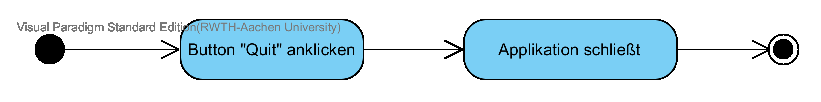
\epsfig{file=Bilder/Beenden1.eps,width=\textwidth}

\textbf{Check Input}
  \begin{itemize}
  \item \textit{Ziel:} Die Applikation will die Gebietsgr\"o\ss e und die numerischen Parameter \"uberpr\"ufen.
  \item \textit{Einordnung:} Hauptfunktion
  \item \textit{Vorbedingung:} Der Nutzer hat auf Run angeklickt.
  \item \textit{Nachbedingung:} Der Use Case "`Check Randfunktionen"' wird gestartet.
  \item \textit{Nachbedingung im Fehlerfall:} Die Applikation zeigt eine Fehlermeldung an und markiert die Stelle, an der sich der Fehler befindet.
  \item \textit{Hauptakteure:} System
  \item \textit{Nebenakteure:}
  \item \textit{Ausl\"oser:} Die Applikation m\"ochte die Gebietsgr\"o\ss e und die numerischen Parameter \"uberpr\"ufen.
  \item \textit{Standardablauf:}
    \begin{enumerate}
    \item Die Applikation pr\"uft, ob die eingegebenen Grenzen der Gebietsgr\"o\ss e g\"ultige double Werte sind.
    \item Die Applikation pr\"uft, ob die obere Grenze xmax gr\"o\ss er als die untere Grenze xmin ist.
    \item Die Applikation pr\"uft, ob die obere Grenze ymax gr\"o\ss er als die untere Grenze ymin ist.
    \item Die Applikation pr\"uft, ob der Abbruchfehler eps gr\"o\ss er 0 und ein double ist.
    \item Die Applikation pr\"uft, ob die maximale Anzahl der Iterationen $max_iteration$, die Anzahl der x-St\"utzstellen n und y-St\"utzstellen m   g\"o\ss er 0 und vom Typ int sind.
  \end{enumerate}
  \item \textit{Verzweigungen:}
    \begin{enumerate}[label=(1a\arabic*)]    
            \item Die Berechnung wird abgebrochen.
	\item Die Applikation zeigt eine Fehlermeldung, falls die Gebietsgr\"o\ss e ung\"ultig ist.(keine Zahl eingegeben oder das Feld leer gelassen)
	\item Das Feld, in dem der Fehler ist, wird markiert.
	\end{enumerate}
	 \begin{enumerate}[label=(2a\arabic*)]    
	 	\item Die Berechnung wird abgebrochen.
		\item Die Applikation zeigt eine Fehlermeldung, falls xmin gr\"o\ss er gleich xmax ist.
		\item Das Feld, in dem der Fehler ist, wird markiert.
	\end{enumerate}
	 \begin{enumerate}[label=(3a\arabic*)]    
	 	\item Die Berechnung wird abgebrochen.
		\item Die Applikation zeigt eine Fehlermeldung, falls ymin gr\"o\ss er gleich ymax ist.\\
		\item Das Feld, in dem der Fehler ist, wird markiert.
	\end{enumerate}
		 \begin{enumerate}[label=(4a\arabic*)]    
		 	\item Die Berechnung wird abgebrochen.
		 \item Die Applikation zeigt eine Fehlermeldung, falls eps ung\"ultig ist.
		 \item Das Feld "`eps edit"' wird markiert.
		 \end{enumerate}
	 \begin{enumerate}[label=(5a\arabic*)]    
	 	\item Die Berechnung wird abgebrochen.
		\item Die Applikation zeigt eine Fehlermeldung, falls ein numerischer Parameter ung\"ultig ist.
		\item Das Feld, in dem der Fehler ist, wird markiert.
    \end{enumerate}
  \end{itemize}

\epsfig{file=Bilder/Check_Input.eps,width=\textwidth}

\textbf{Check Randfunktionen}
  \begin{itemize}
  \item \textit{Ziel:} Das System will die Randfunktionen \"uberpr\"ufen.
  \item \textit{Einordnung:} Hauptfunktion
  \item \textit{Vorbedingung:} Use Case Check Input wurde erfolgreich durchgef\"uhrt.
  \item \textit{Nachbedingung:} Die Berechnung wird durchgef\"uhrt.
  \item \textit{Nachbedingung im Fehlerfall:} Die Applikation zeigt eine Fehlermeldung an und markiert die Stelle, an der sich der Fehler befindet.
  \item \textit{Hauptakteure:} System
  \item \textit{Nebenakteure:}
  \item \textit{Ausl\"oser:} Der Nutzer hat auf 'run' gedr\"uckt und UC Check Input war erfolgreich.
  \item \textit{Standardablauf:}
    \begin{enumerate}
    \item Das System pr\"uft, ob weniger als 2 Variablen vorhanden sind.
    \item Das System pr\"uft, ob die Randfunktionen g\"ultig sind.
  \end{enumerate}
  \item \textit{Verzweigungen:}
    \begin{enumerate}[label=(1a\arabic*)]
	\item Das System zeigt eine Fehlermeldung, falls mehr als 2 Variablen vorhanden sind.
	\item Die Berechnung wird abgebrochen.
	\end{enumerate}
	 \begin{enumerate}[label=(2a\arabic*)]
	\item Das System zeigt eine Fehlermeldung, falls die Randfunktion ung\"ultig ist.
	\item Die Berechnung wird abgebrochen.
    \end{enumerate}
  \end{itemize}

\epsfig{file=Bilder/Check_Randfunktionen.eps,width=\textwidth}

\textbf{Einstellungen laden}
  \begin{itemize}
  \item \textit{Ziel:} Der Nutzer will vorher gespeicherte Einstellungen im .setup Format laden.
  \item \textit{Einordnung:} Hauptfunktion
  \item \textit{Vorbedingung:} Die Applikation wurde gestartet
  \item \textit{Nachbedingung:} Das System l\"adt eine Datei mit den gespeicherten Daten und das MainWindow wird angezeigt.
    \item \textit{Nachbedingung im Fehlerfall:} Nichts wird ver\"andert.
  \item \textit{Hauptakteure:} Nutzer
  \item \textit{Nebenakteure:} System
  \item \textit{Ausl\"oser:} Der Nutzer m\"ochte eine vorher eingestellte gespeicherte Einstellung im .setup Format laden.
    \item \textit{Standardablauf:}
    \begin{enumerate}
    \item Der Nutzer klickt mit der linken Maustaste auf dem Button "Einstellungen laden" an.
    \item Das System zeigt das Dialogfenster an.
    \item Der Nutzer sucht und w\"ahlt einen Ladepfad aus.
    \item Der Nutzer markiert die Datei im .setup Format.
    \item Der Nutzer klickt auf den Button "` \"Offnen"'.
    \item Das System zeigt die gespeicherten Daten im Anzeige Tab an.
  \end{enumerate}
  \item \textit{Verzweigungen:}
    \begin{enumerate}[label=(3\arabic*)]
\item Es befindet sich keine vorher gespeicherte Einstellungsdatei.
    \end{enumerate}
  \end{itemize}

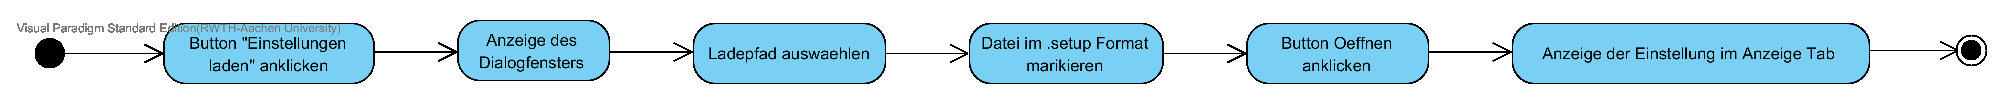
\epsfig{file=Bilder/Einstellungen_laden.eps,width=\textwidth}

\textbf{Einstellungen speichern}
  \begin{itemize}
  \item \textit{Ziel:} Der Nutzer will die eingegebenen Einstellungen speichern.
  \item \textit{Einordnung:} Hauptfunktion
  \item \textit{Vorbedingung:} Die Applikation wurde gestartet.
  \item \textit{Nachbedingung:} Das System erstellt eine .setup Datei mit den gespeicherten Daten und das MainWindow wird angezeigt.
    \item \textit{Nachbedingung im Fehlerfall:}
  \item \textit{Hauptakteure:} Nutzer
  \item \textit{Nebenakteure:} System
  \item \textit{Ausl\"oser:} Der Nutzer m\"ochte die eingegebenen Einstellungen speichern.
    \item \textit{Standardablauf:}
    \begin{enumerate}
    \item Der Nutzer klickt mit der linken Maustaste auf "Einstellungen speichern".
    \item Das System zeigt das Dialogfenster an.
    \item Der Nutzer w\"ahlt den Speicherpfad aus.
    \item Der Nutzer gibt \"uber die Tastatur den Dateinamen ein.
    \item Der Nutzer klickt auf den Button "Speichern".
    \item Das System speichert die eingegebenen  Einstellungen im angegebenen Verzeichnis als .setup Datei
  \end{enumerate}
  \end{itemize}

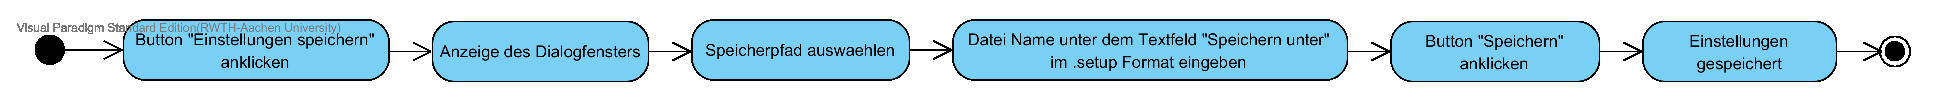
\epsfig{file=Bilder/Einstellungen_speichern_1.eps,width=\textwidth}

\textbf{Ergebnis laden}
  \begin{itemize}
  \item \textit{Ziel:} Der Nutzer will eine vorher gespeicherte Ergebnisdatei im .surface Format laden.
  \item \textit{Einordnung:} Hauptfunktion
  \item \textit{Vorbedingung:} Die Applikation wurde gestartet
  \item \textit{Nachbedingung:} Das System l\"adt die gespeicherten Ergebnisdaten und zeigt sie im Anzeige Tab an.
    \item \textit{Nachbedingung im Fehlerfall:} Es wird nichts ver\"andert.
  \item \textit{Hauptakteure:} Nutzer
  \item \textit{Nebenakteure:} System
  \item \textit{Ausl\"oser:} Der Nutzer m\"ochte eine vorher gespeicherte Ergebnisdatei im .surface Format laden.
    \item \textit{Standardablauf:}
    \begin{enumerate}
    \item Der Nutzer klickt mit der linken Maustaste auf den Button "Ergebnis laden".
    \item Das System zeigt das Dialogfenster an.
    \item Der Nutzer sucht und w\"ahlt den Ladepfad aus.
    \item Der Nutzer markiert mit der linken Maustaste die .surface Datei.
    \item Der Nutzer klickt mit der linken Maustaste auf den Button \"Offnen.
    \item Das System zeigt die Ergebnisdaten im Anzeige Tab an.   
  \end{enumerate}
  \item \textit{Verzweigungen:}
    \begin{enumerate}[label=(3\arabic*)]
\item Es befindet sich keine vorher gespeicherte Einstellungsdatei.
    \end{enumerate}
  \end{itemize}
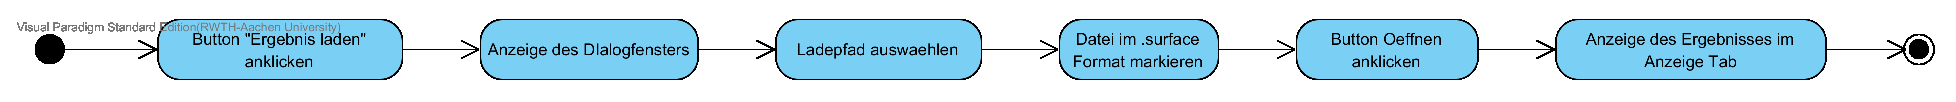
\epsfig{file=Bilder/Ergebnis_laden_1.eps,width=\textwidth}
\textbf{Ergebnis speichern}
  \begin{itemize}
  \item \textit{Ziel:} Der Nutzer will die Ergebnisdaten speichern.
  \item \textit{Einordnung:} Hauptfunktion
  \item \textit{Vorbedingung:} Die Applikation wurde gestartet.
  \item \textit{Nachbedingung:} Das System erstellt eine .surface Datei mit den gespeicherten Daten, den numerischen Parametern und der Gebietsgr\"o\ss e. Das MainWindow wird angezeigt.
    \item \textit{Nachbedingung im Fehlerfall:} Das System zeigt eine Fehlermeldung, weil noch keine Berechnung durchgef\"uhrt wurde.
      \item \textit{Hauptakteure:} Nutzer
  \item \textit{Nebenakteure:} System
  \item \textit{Ausl\"oser:} Der Nutzer m\"ochte die Ergebnisdaten speichern.
    \item \textit{Standardablauf:}
    \begin{enumerate}
    \item Der Nutzer klickt mit der linken Maustaste "Ergebnis speichern" an.
    \item Das System pr\"uft, ob eine Berechnung schon durchgef\"uhrt wurde.
    \item Das System zeigt das Dialogfenster an.
    \item Der Nutzer sucht und w\"ahlt einen Pfad aus.
	\item Der Nutzer gibt \"uber die Tastatur den Dateinamen ein.
	\item Der Nutzer klickt auf den Button "Speichern".
	\item Das System speichert die Ergebnisdaten als .surface Datei
  \end{enumerate}
  \item \textit{Verzweigungen:}
    \begin{enumerate}[label=(2\arabic*)]
\item Das System zeigt eine Fehlermeldung an, da zuvor keine Berechnung durchgef\"uhrt wurde.
\item Der UC Ergebnis speichern wird beendet.
    \end{enumerate}
  \end{itemize}
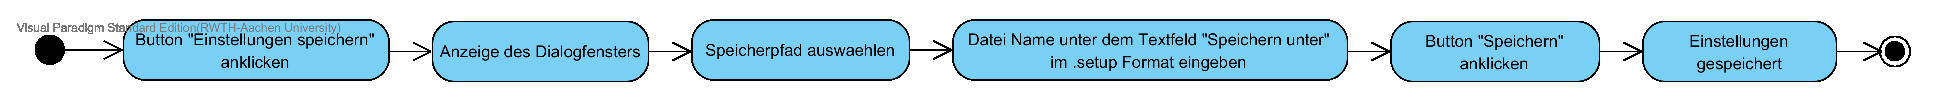
\epsfig{file=Bilder/Einstellungen_speichern_1.eps,width=\textwidth}
\textbf{Gebietsgr\"o\ss e \"Andern}
  \begin{itemize}
  \item \textit{Ziel:} Der Nutzer will einen Wert der Gebietsgr\"o\ss e \"andern.
  \item \textit{Einordnung:} Hauptfunktion
  \item \textit{Vorbedingung:} Die Applikation wurde gestartet und der Tab 'Einstellungen' im MainWindow wird angezeigt.
  \item \textit{Nachbedingung:} Die Gebietsgr\"o\ss e wurde ver\"andert.
  \item \textit{Nachbedingung im Fehlerfall:} 
  \item \textit{Hauptakteure:} Nutzer
  \item \textit{Nebenakteure:} System
  \item \textit{Ausl\"oser:} Der Nutzer m\"ochte einen Wert der Gebietsgr\"o\ss e \"andern.
  \item \textit{Standardablauf:}
    \begin{enumerate}
    \item Der Nutzer klickt mit der linken Maustaste auf beliebiges Feld der Gebietsgr\"o\ss e.
    \item Der Nutzer gibt \"uber die Tastatur den neuen Wert der Gebietsgr\"o\ss e ein.
  \end{enumerate}
  \end{itemize}

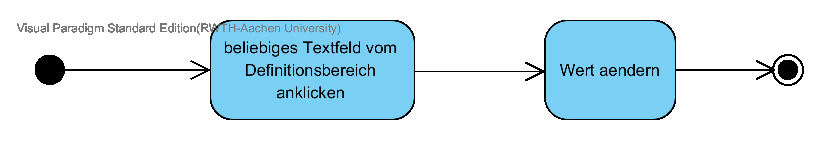
\epsfig{file=Bilder/Gebietsgroesse_aendern1.eps,width=\textwidth}
\textbf{Numerische Parameter \"Andern}
  \begin{itemize}
  \item \textit{Ziel:} Der Nutzer will einen  numerischen Parameter \"andern.
  \item \textit{Einordnung:} Hauptfunktion
  \item \textit{Vorbedingung:} Die Applikation wurde gestartet und der Tab 'Setting' im MainWindow wird angezeigt.
  \item \textit{Nachbedingung:} Der numerische Parameter wurde ver\"andert.
  \item \textit{Nachbedingung im Fehlerfall:} 
  \item \textit{Hauptakteure:} Nutzer
  \item \textit{Nebenakteure:} System
  \item \textit{Ausl\"oser:} Der Nutzer m\"ochte einen  numerischen Parameter \"andern.
  \item \textit{Standardablauf:}
    \begin{enumerate}
    \item Der Nutzer klickt mit der linken Maustaste auf beliebiges Feld der numerischen Parameter. 
    \item Der Nutzer gibt \"uber die Tastatur den neuen numerischen Wert ein.
  \end{enumerate}
  \end{itemize}
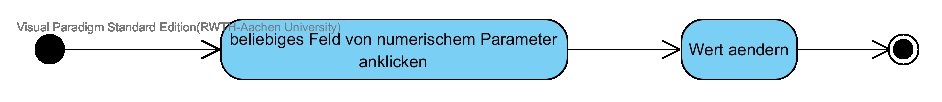
\epsfig{file=Bilder/Numerische_Parameter_aendern.eps,width=\textwidth}
\textbf{Randfunktionen \"Andern}
  \begin{itemize}
  \item \textit{Ziel:} Der Nutzer will eine Randfunktion \"andern.
  \item \textit{Einordnung:} Hauptfunktion
  \item \textit{Vorbedingung:} Die Applikation wurde gestartet und der Tab 'Setting' im MainWindow wird angezeigt.
  \item \textit{Nachbedingung:} Die Randfunktion wurde ver\"andert.
  \item \textit{Nachbedingung im Fehlerfall:}  
  \item \textit{Hauptakteure:} Nutzer
  \item \textit{Nebenakteure:} System
  \item \textit{Ausl\"oser:} Der Nutzer m\"ochte eine Randfunktion \"andern.
  \item \textit{Standardablauf:}
    \begin{enumerate}
    \item Der Nutzer klickt mit der linken Maustaste auf beliebiges Feld der Randfunktionen an.
    \item Der Nutzer gibt \"uber die Tastatur die neue Randfunktion ein. 
  \end{enumerate}
  \end{itemize}
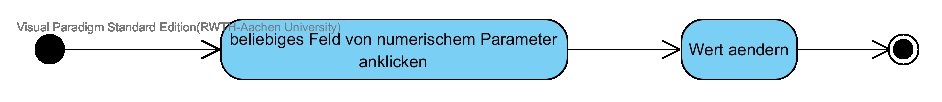
\epsfig{file=Bilder/Numerische_Parameter_aendern.eps,width=\textwidth}
\textbf{run}
  \begin{itemize}
  \item \textit{Ziel:} Der Nutzer will die Berechnung der Minimalfl\"ache durchf\"uhren und anzeigen.
  \item \textit{Einordnung:} Hauptfunktion
  \item \textit{Vorbedingung:} Die Applikation wurde gestartet, alle numerische Parameter, Randfunktionen und Gebietsgr\"o\ss e sind eingegeben.
  \item \textit{Nachbedingung:} Die Applikation zeigt die berechneten Minimalfl\"achen im Tab "`Anzeige"' an.
    \item \textit{Nachbedingung im Fehlerfall:} Es wird eine Fehlermeldung angezeigt.
  \item \textit{Hauptakteure:} Nutzer
  \item \textit{Nebenakteure:} System
  \item \textit{Ausl\"oser:} Der Nutzer will die Berechnung starten.
    \item \textit{Standardablauf:}
    \begin{enumerate}
    \item Der Nutzer klickt mit der linken Maustaste auf den Button 'Run'.
    \item UC "`Check Input"'
    \item UC "`Check Randfunktionen"'
    \item Die Applikation wechselt den Tab auf "`Konsolenausgabe"'.
    \item Die Applikation startet mit den gegeben Einstellungen die Berechnung der Minimalf\"achen.
    \item Die Applikation zeigt den Fortschritt der Berechnung auf der Benutzeroberfl\"ache an.
    \item Die Applikation schliesst die Berechnung ab.
    \item Die Applikation wechselt den Tab auf "`Anzeige"'
    \item Die Applikation zeigt die berechnete Minimalfl\"ache an.
  \end{enumerate}
  \item \textit{Verzweigungen:}
      \begin{enumerate}[label=(2a\arabic*)]
  \item Der UC "`Check Input"' ist fehlerhaft, die Applikation zeigt eine Fehlermeldung an und stoppt die Berechnung.
      \end{enumerate}
    \begin{enumerate}[label=(3a\arabic*)]
  \item Der UC "`Check Randfunktionen"' ist fehlerhaft, die Applikation zeigt eine Fehlermeldung an und stoppt die Berechnung.
    \end{enumerate}
    \begin{enumerate}[label=(7a\arabic*)]
    \item Die Berechnung ist nicht konvergiert, die Applikation zeigt auf der "`Konsolenausgabe"' eine Fehlermeldung an.
     \item Die Applikation wechselt den Tab auf "`Anzeige"'
     \item Die Applikation zeigt die nicht vollst\"andig berechnete Minimalfl\"ache an.
        \end{enumerate}
  \end{itemize}
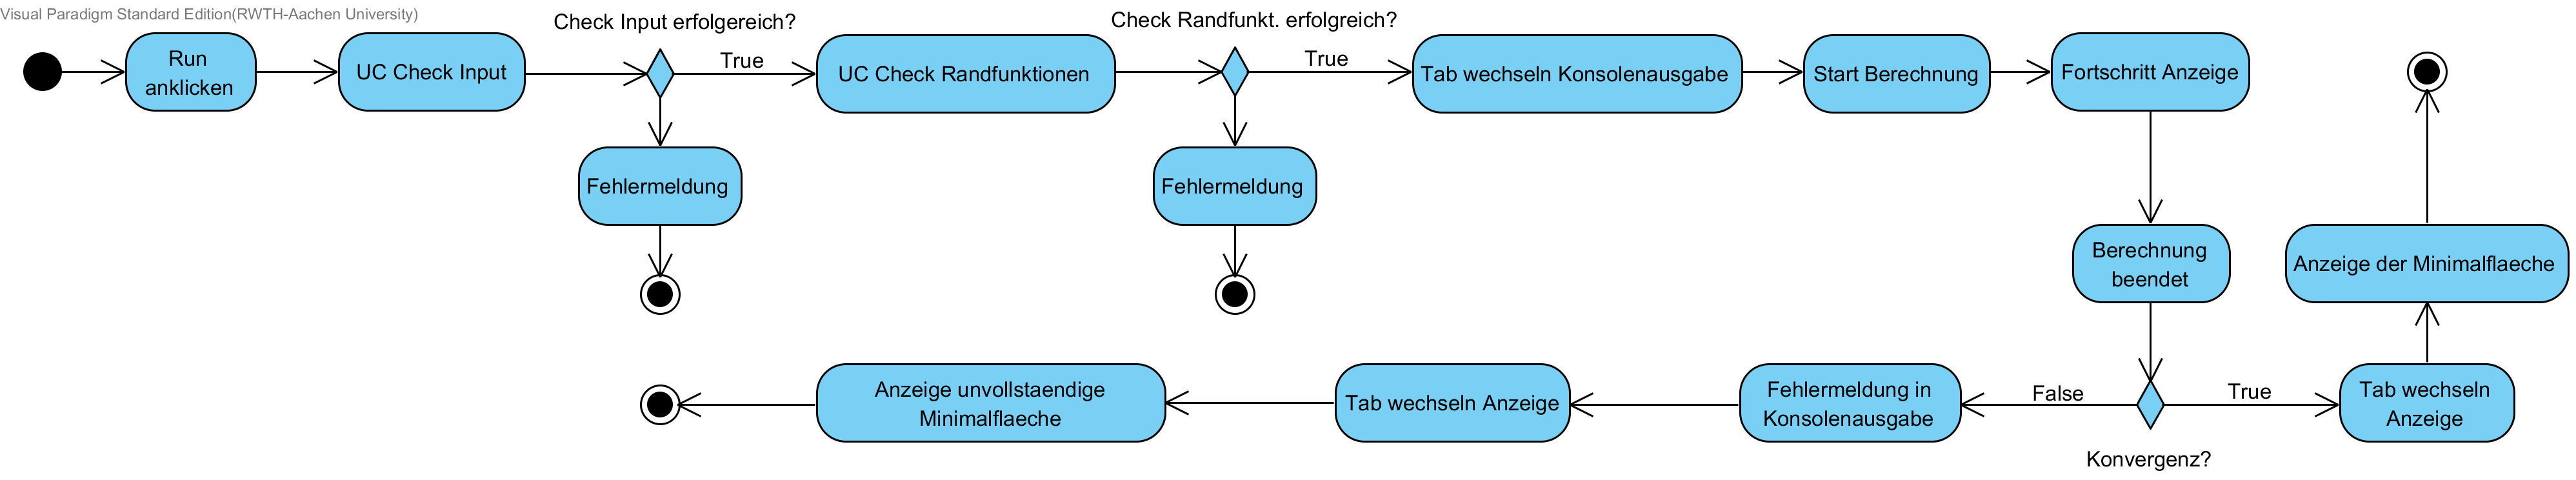
\epsfig{file=Bilder/Run1.eps,width=\textwidth}
\textbf{Tab wechseln}
  \begin{itemize}
  \item \textit{Ziel:} Der Nutzer will zu einem anderen Tab wechseln.
  \item \textit{Einordnung:} Hauptfunktion
  \item \textit{Vorbedingung:} Die Applikation wurde erfolgreich gestartet.
  \item \textit{Nachbedingung:} Die Applikation zeigt den neuen Tab an.
  \item \textit{Nachbedingung im Fehlerfall:} 
  \item \textit{Hauptakteure:} Nutzer
  \item \textit{Nebenakteure:} System
  \item \textit{Ausl\"oser:} Der Nutzer m\"ochte auf einen anderen Tab wechseln.
  \item \textit{Standardablauf:}
    \begin{enumerate}
     \item Der Nutzer klickt mit der linken Maustaste auf den gew\"unschten Tab.
    \item Die Applikation wechselt den Tab und zeigt den ausgew\"ahlten Tab an.
  \end{enumerate}
  \end{itemize}
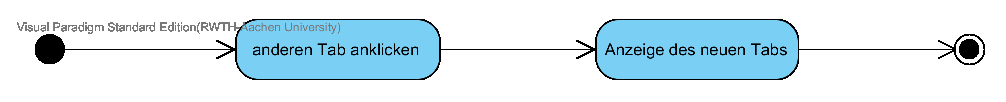
\epsfig{file=Bilder/Tab_wechseln1.eps,width=\textwidth}


\subsection{Funktionale Anforderung}
\begin{itemize}
\item Anzeigen einer Benutzeroberfl\"ache
\item Speichern der Einstellungen
\item Laden der Einstellungen
\item Speichern der Ergebnisse
\item Laden der Ergebnisse
\item M\"oglicher Wechsel zwischen drei Tabs. Funktionen des ersten Tabs (Einstellungen):
	\begin{enumerate}
	\item Eingabe der Anzahl der St\"utzstellen in X- und Y-Richtung
	\item Eingabe der Randfunktionen
	\item Eingabe des Abbruchfehlers
	\item Eingabe der Anzahl der maximalen Iterationen
	\item \"Anderung des Gebietes
	\item Run Button
	\item Quit Button
	\end{enumerate}
\item Funktionen des zweiten Tabs (Konsolenausgabe):
	\begin{enumerate}
	\item Anzeigen des Fortschrittes
	\item Anzeigen von Fehlermeldungen
	\end{enumerate}
\item Funktionen des dritten Tabs (Anzeige):
	\begin{enumerate}
	\item Graphische Darstellung der berechneten Minimalfl\"achen
	\item Plot: variabler viewpoint
	\item Instation\"are Anzeige des derzeitigen Ergebnisses w\"ahrend der Berechnung
	\end{enumerate}
\item Test auf G\"ultigkeit des Gebietsbereiches
\item Test auf ganze Zahl der Anzahl der St\"utzstellen.
\end{itemize}
\subsection{Nicht Funktionale Anforderung}
\begin{itemize}
\item Eingabe der Zahlen durch Tastatur
\item Skalierung des Hauptfensters bei unterschiedlichen Aufl\"osungen.
		\item Skalierung des Hauptfensters bei unterschiedlichen Aufl\"osungen
		\item Erzeugung von korrekten Ergebnissen
		\item Intuitive Bedienbarkeit
		\item Plattformunabh\"angig
		\item Effiziente Berechnung
\end{itemize}


\section{Begriffsanalyse}

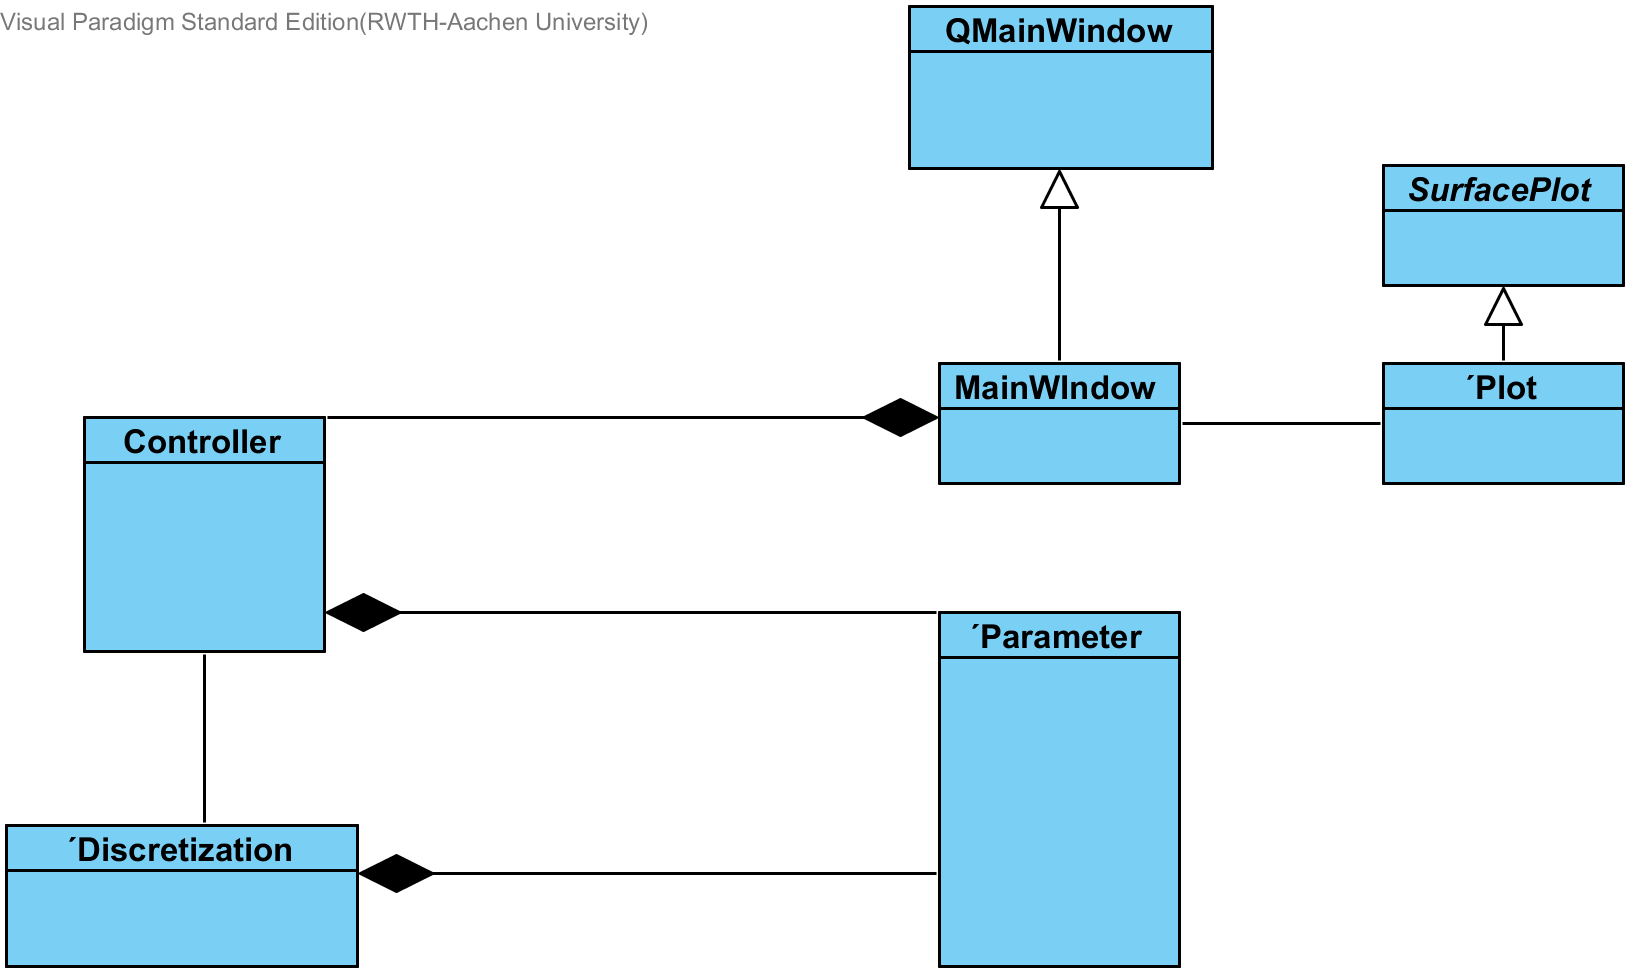
\epsfig{file=Bilder/Begriffsmodel.eps,width=\textwidth}



\noindent \textbf{Klassenkadidaten} 
\begin{itemize}
	\item \textbf{Diskretisierung}
	\item \textbf{Eingabebereich}
	\item \textbf{Ausgabebereich}
	\item \textbf{Main Window}
	\item Textfeld f\"ur Eingabe
	\item Button
	\item Radiobutton
	\item Dialogfenster
	\item Fehlermeldung(durch main implementiert)
	\item Berechnungsparameter
	\item Randwert
	\item Gebietsgr\"o\ss e
\end{itemize}






\chapter{Entwurf}
\label{ch:3}

\section{Klassendiagramm}
\label{sec:3.1}
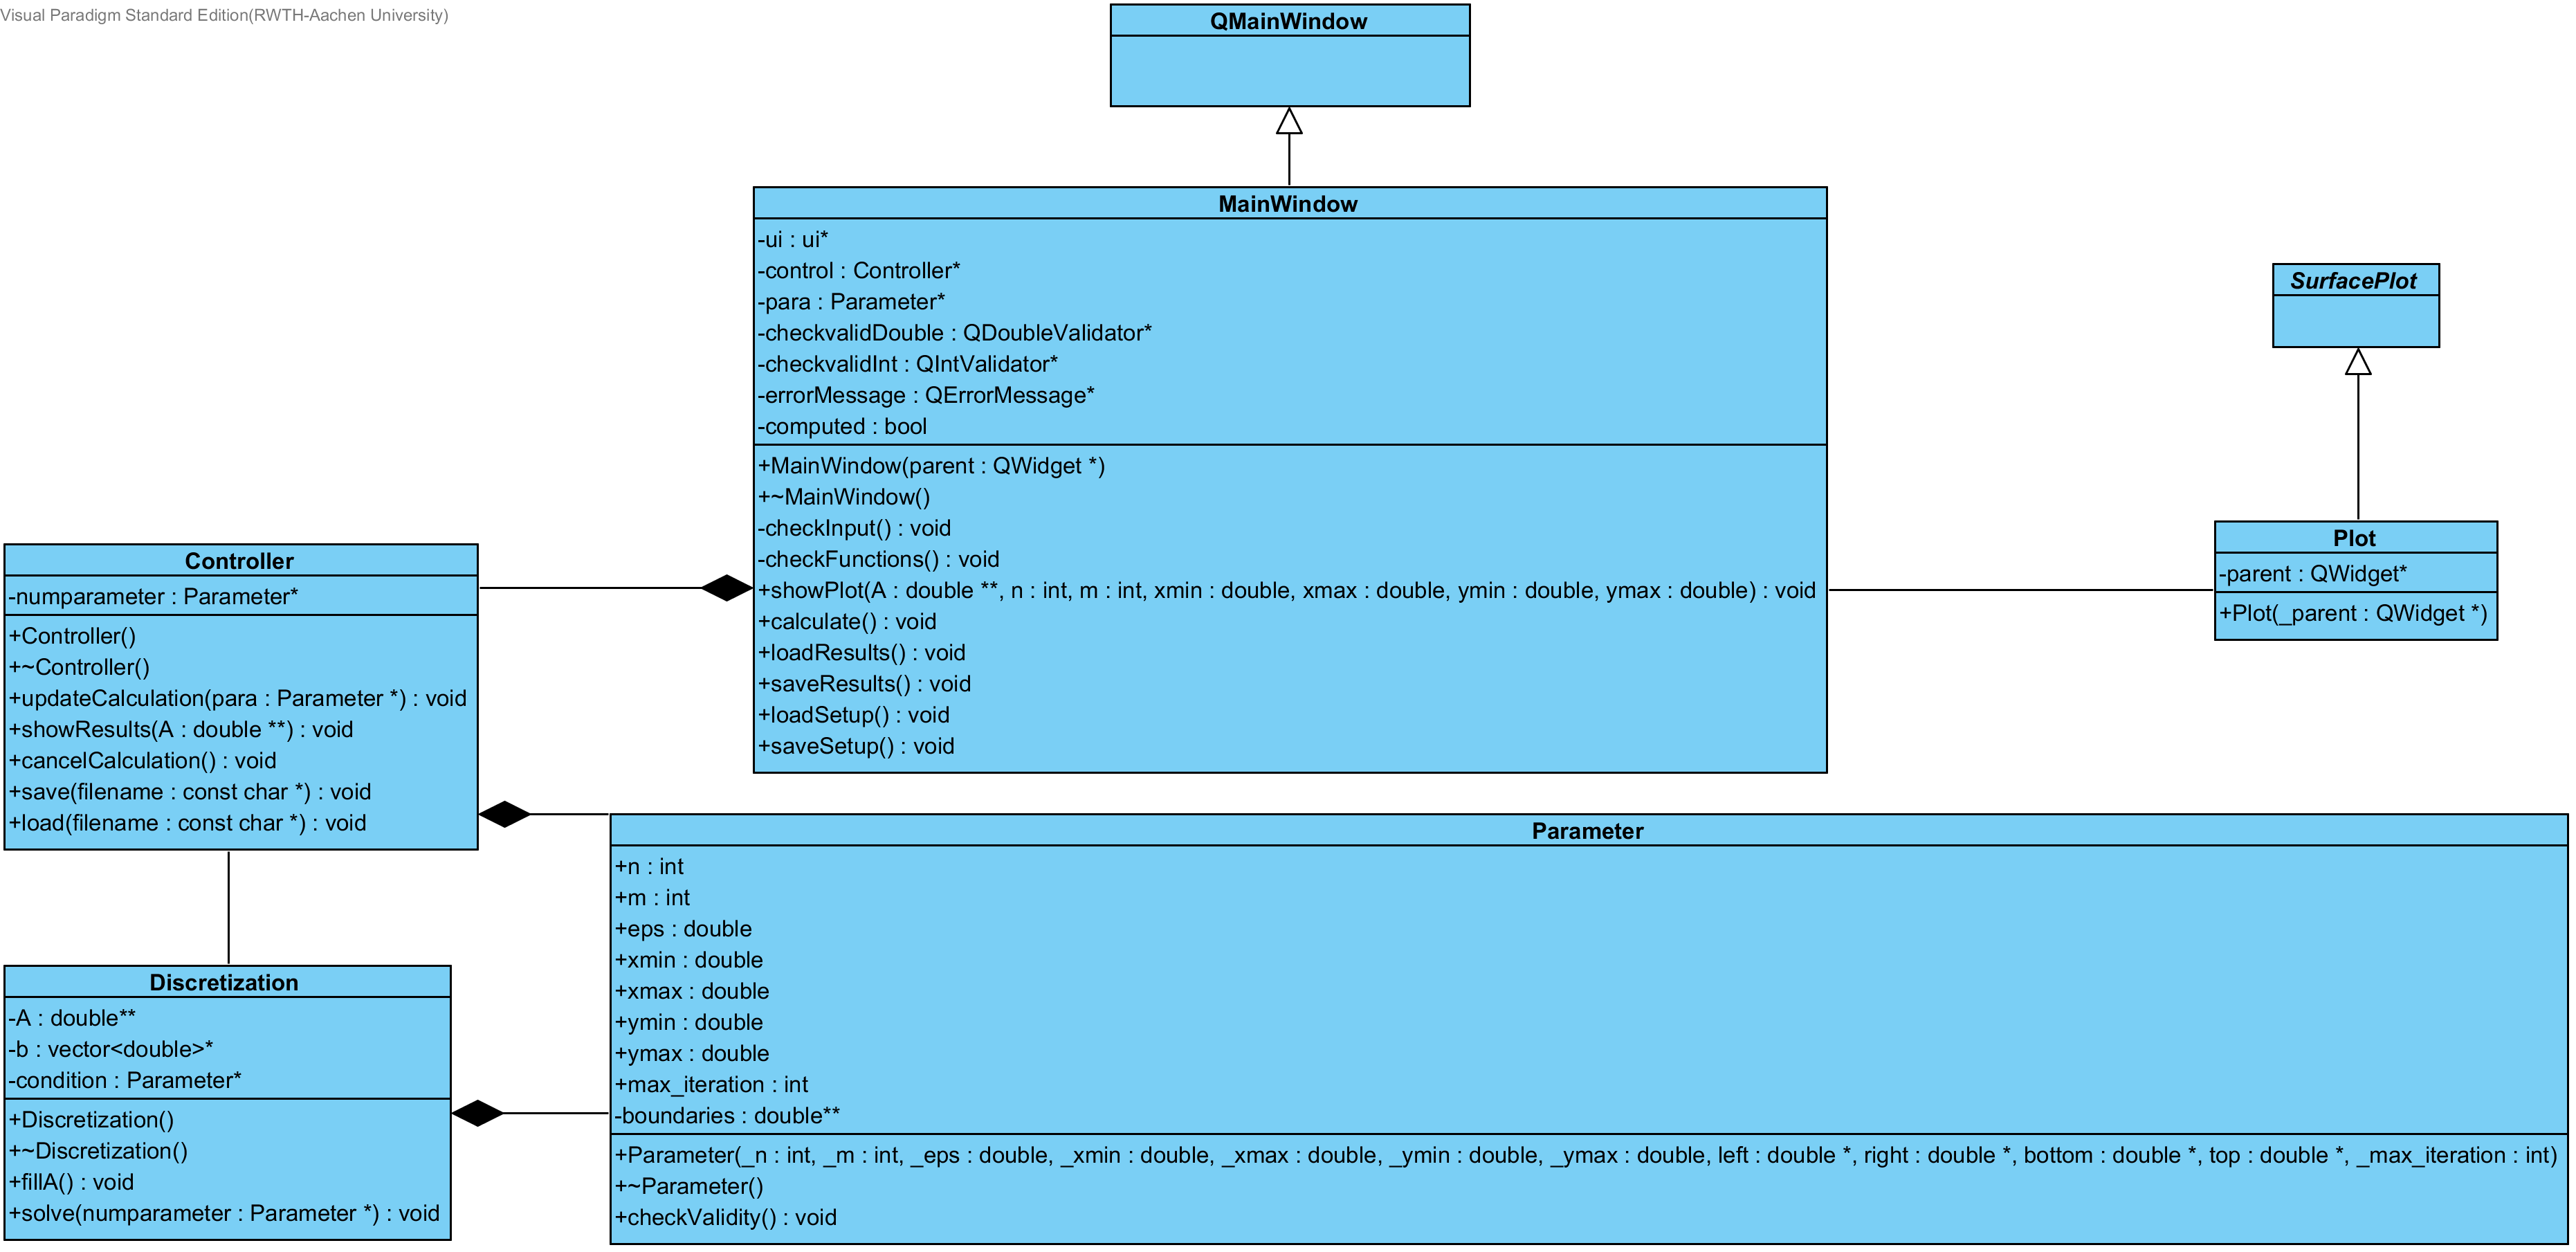
\epsfig{file=Bilder/Klassendiagramm.eps,width=\textwidth}

\section{Dynamik}
\label{sec:3.2}

\subsection{Sequenzdiagramme}

 \textbf{Beenden} \\ \newline 
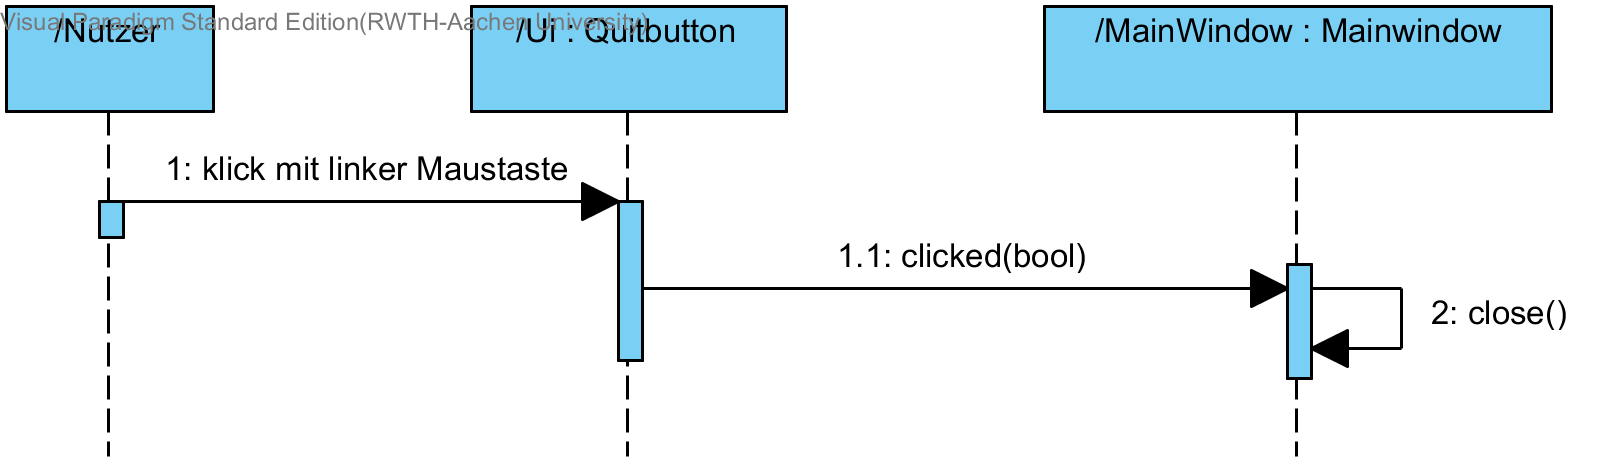
\epsfig{file=Bilder/Beenden.eps,width=\textwidth}
\newline \newline
 \textbf{Check Input} \\
\epsfig{file=Bilder/CheckInput.eps,width=\textwidth}
\newline \newline
 \textbf{Check Randfunktionen} \\
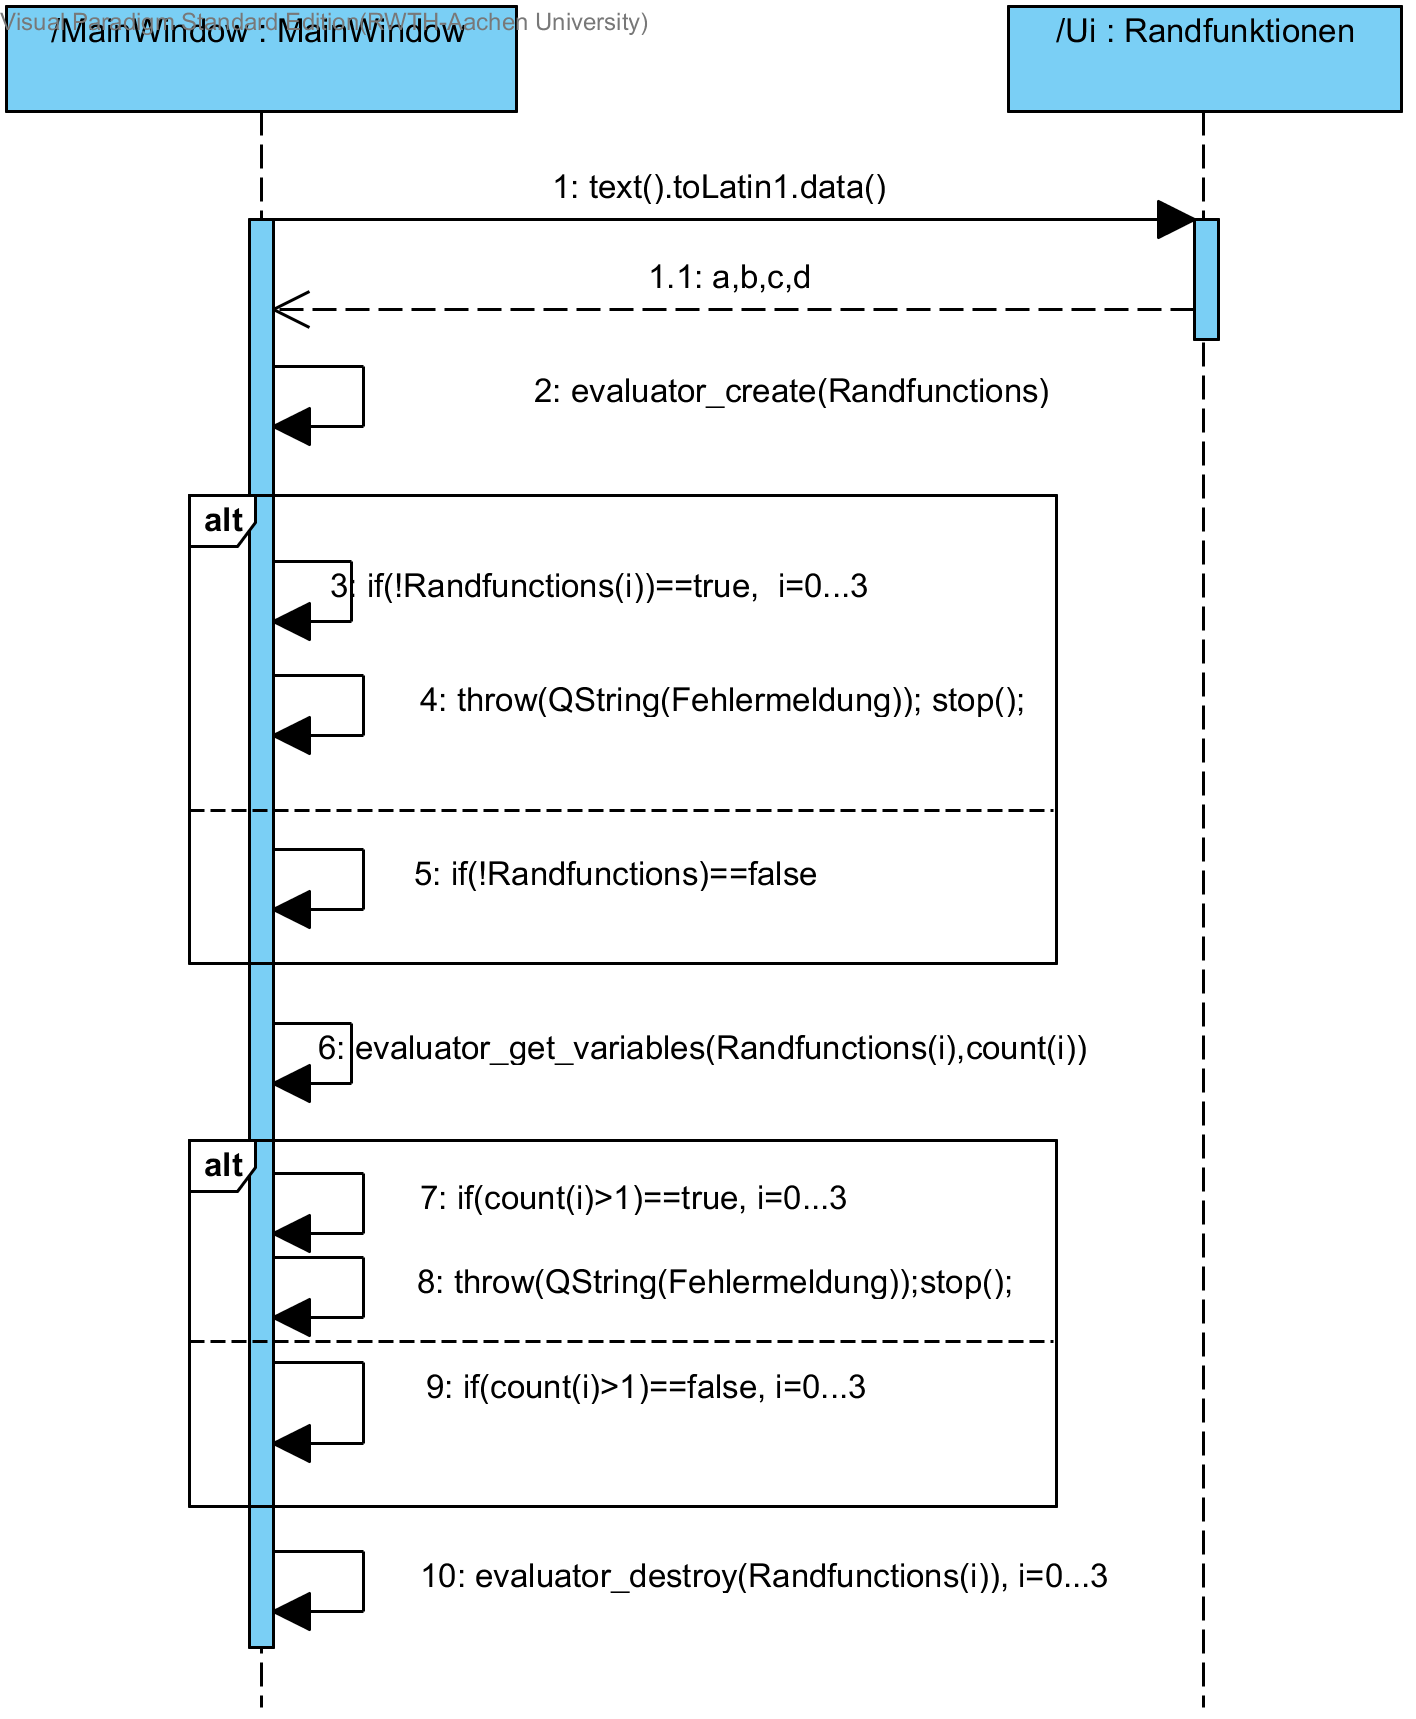
\epsfig{file=Bilder/checkRandfunktionen.eps,width=\textwidth}
\newline \newline
 \textbf{Einstellungen laden} \\
 \newline \newline
\epsfig{file=Bilder/Einstellungen_Laden_1.eps,width=\textwidth}
 \textbf{Einstellungen speichern} \\ \newline
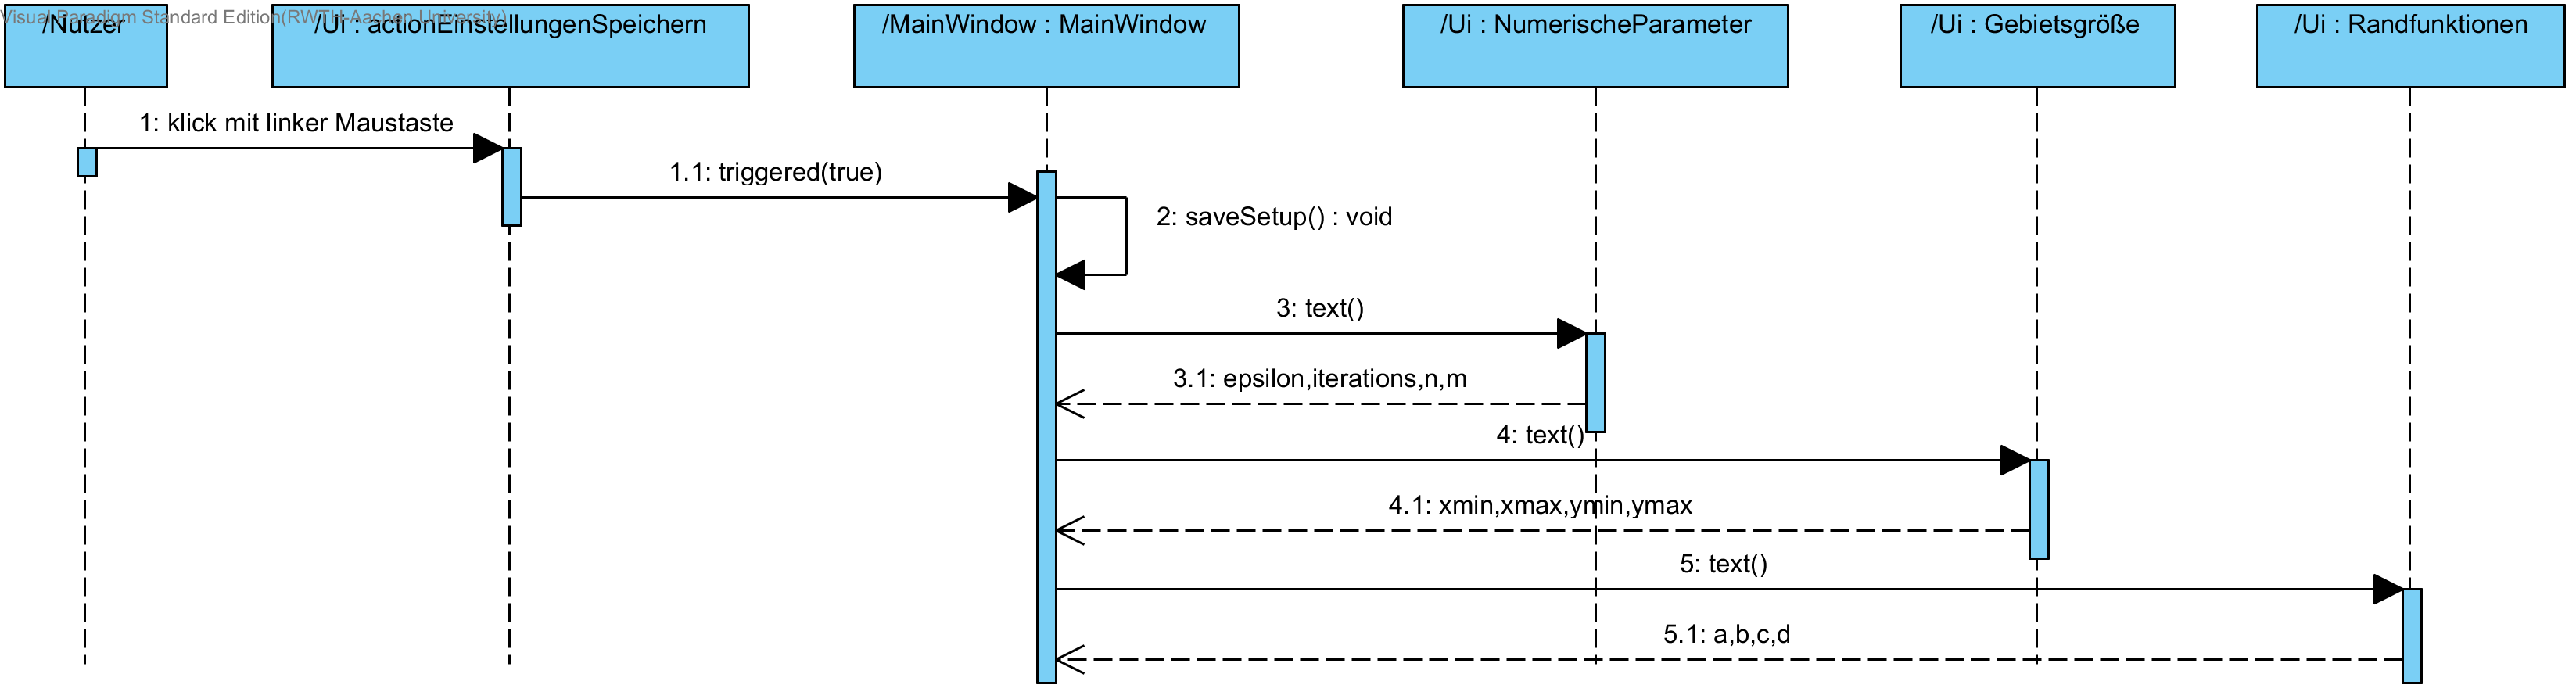
\epsfig{file=Bilder/Einstellungen_Speichern.eps,width=\textwidth}
 \textbf{Ergebnis laden} \\ \newline
\epsfig{file=Bilder/Ergebnis_Laden.eps,width=\textwidth}
 \textbf{Ergebnis speichern} \\ \newline
\epsfig{file=Bilder/Ergebnis_Speichern.eps,width=\textwidth}
 \textbf{Gebietsgr\"o\ss e \"andern} \\ \newline
\epsfig{file=Bilder/Gebietsgroesse_aendern.eps,width=\textwidth}
 \textbf{Numerische Parameter \"andern} \\ \newline
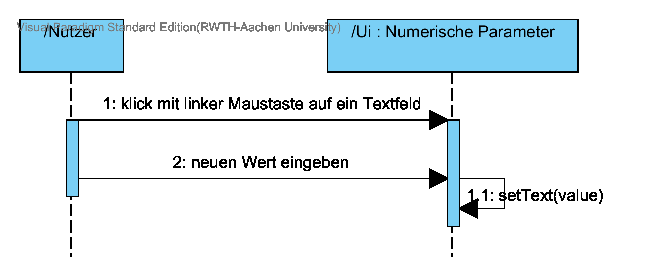
\epsfig{file=Bilder/NumerischeParameterAendern.eps,width=\textwidth}
 \textbf{Randfunktionen \"andern} \\ \newline
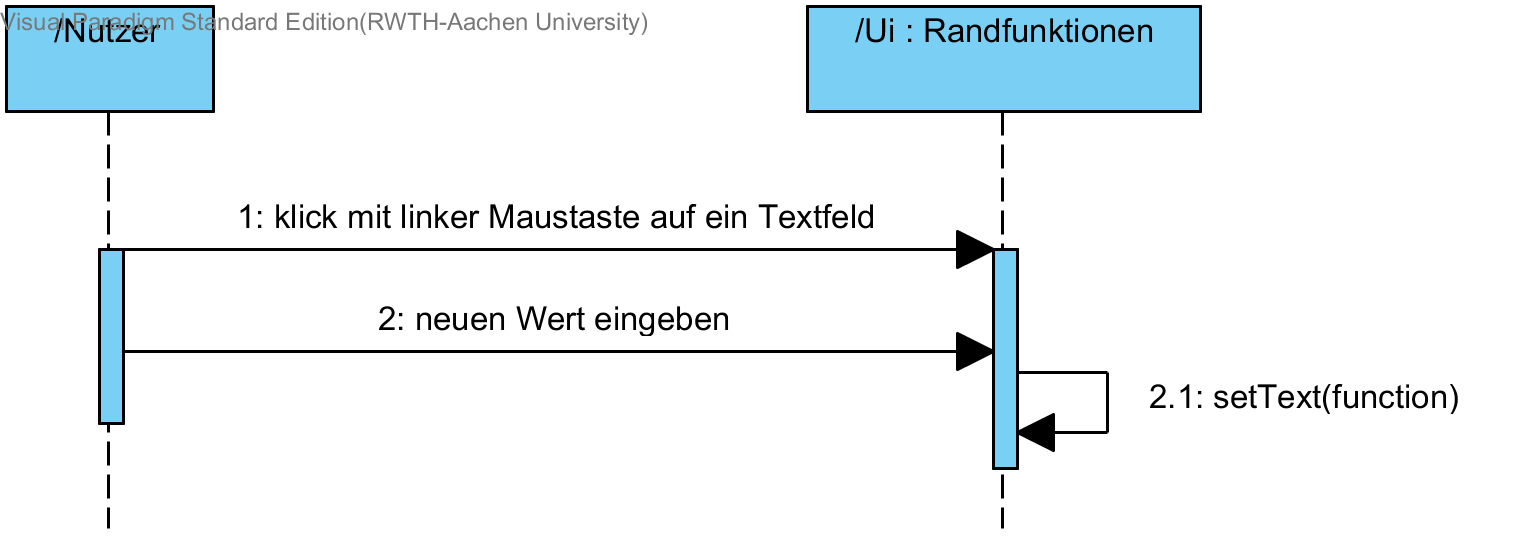
\epsfig{file=Bilder/RandfunktionenAendern.eps,width=\textwidth}
 \textbf{Run} \\ \newline
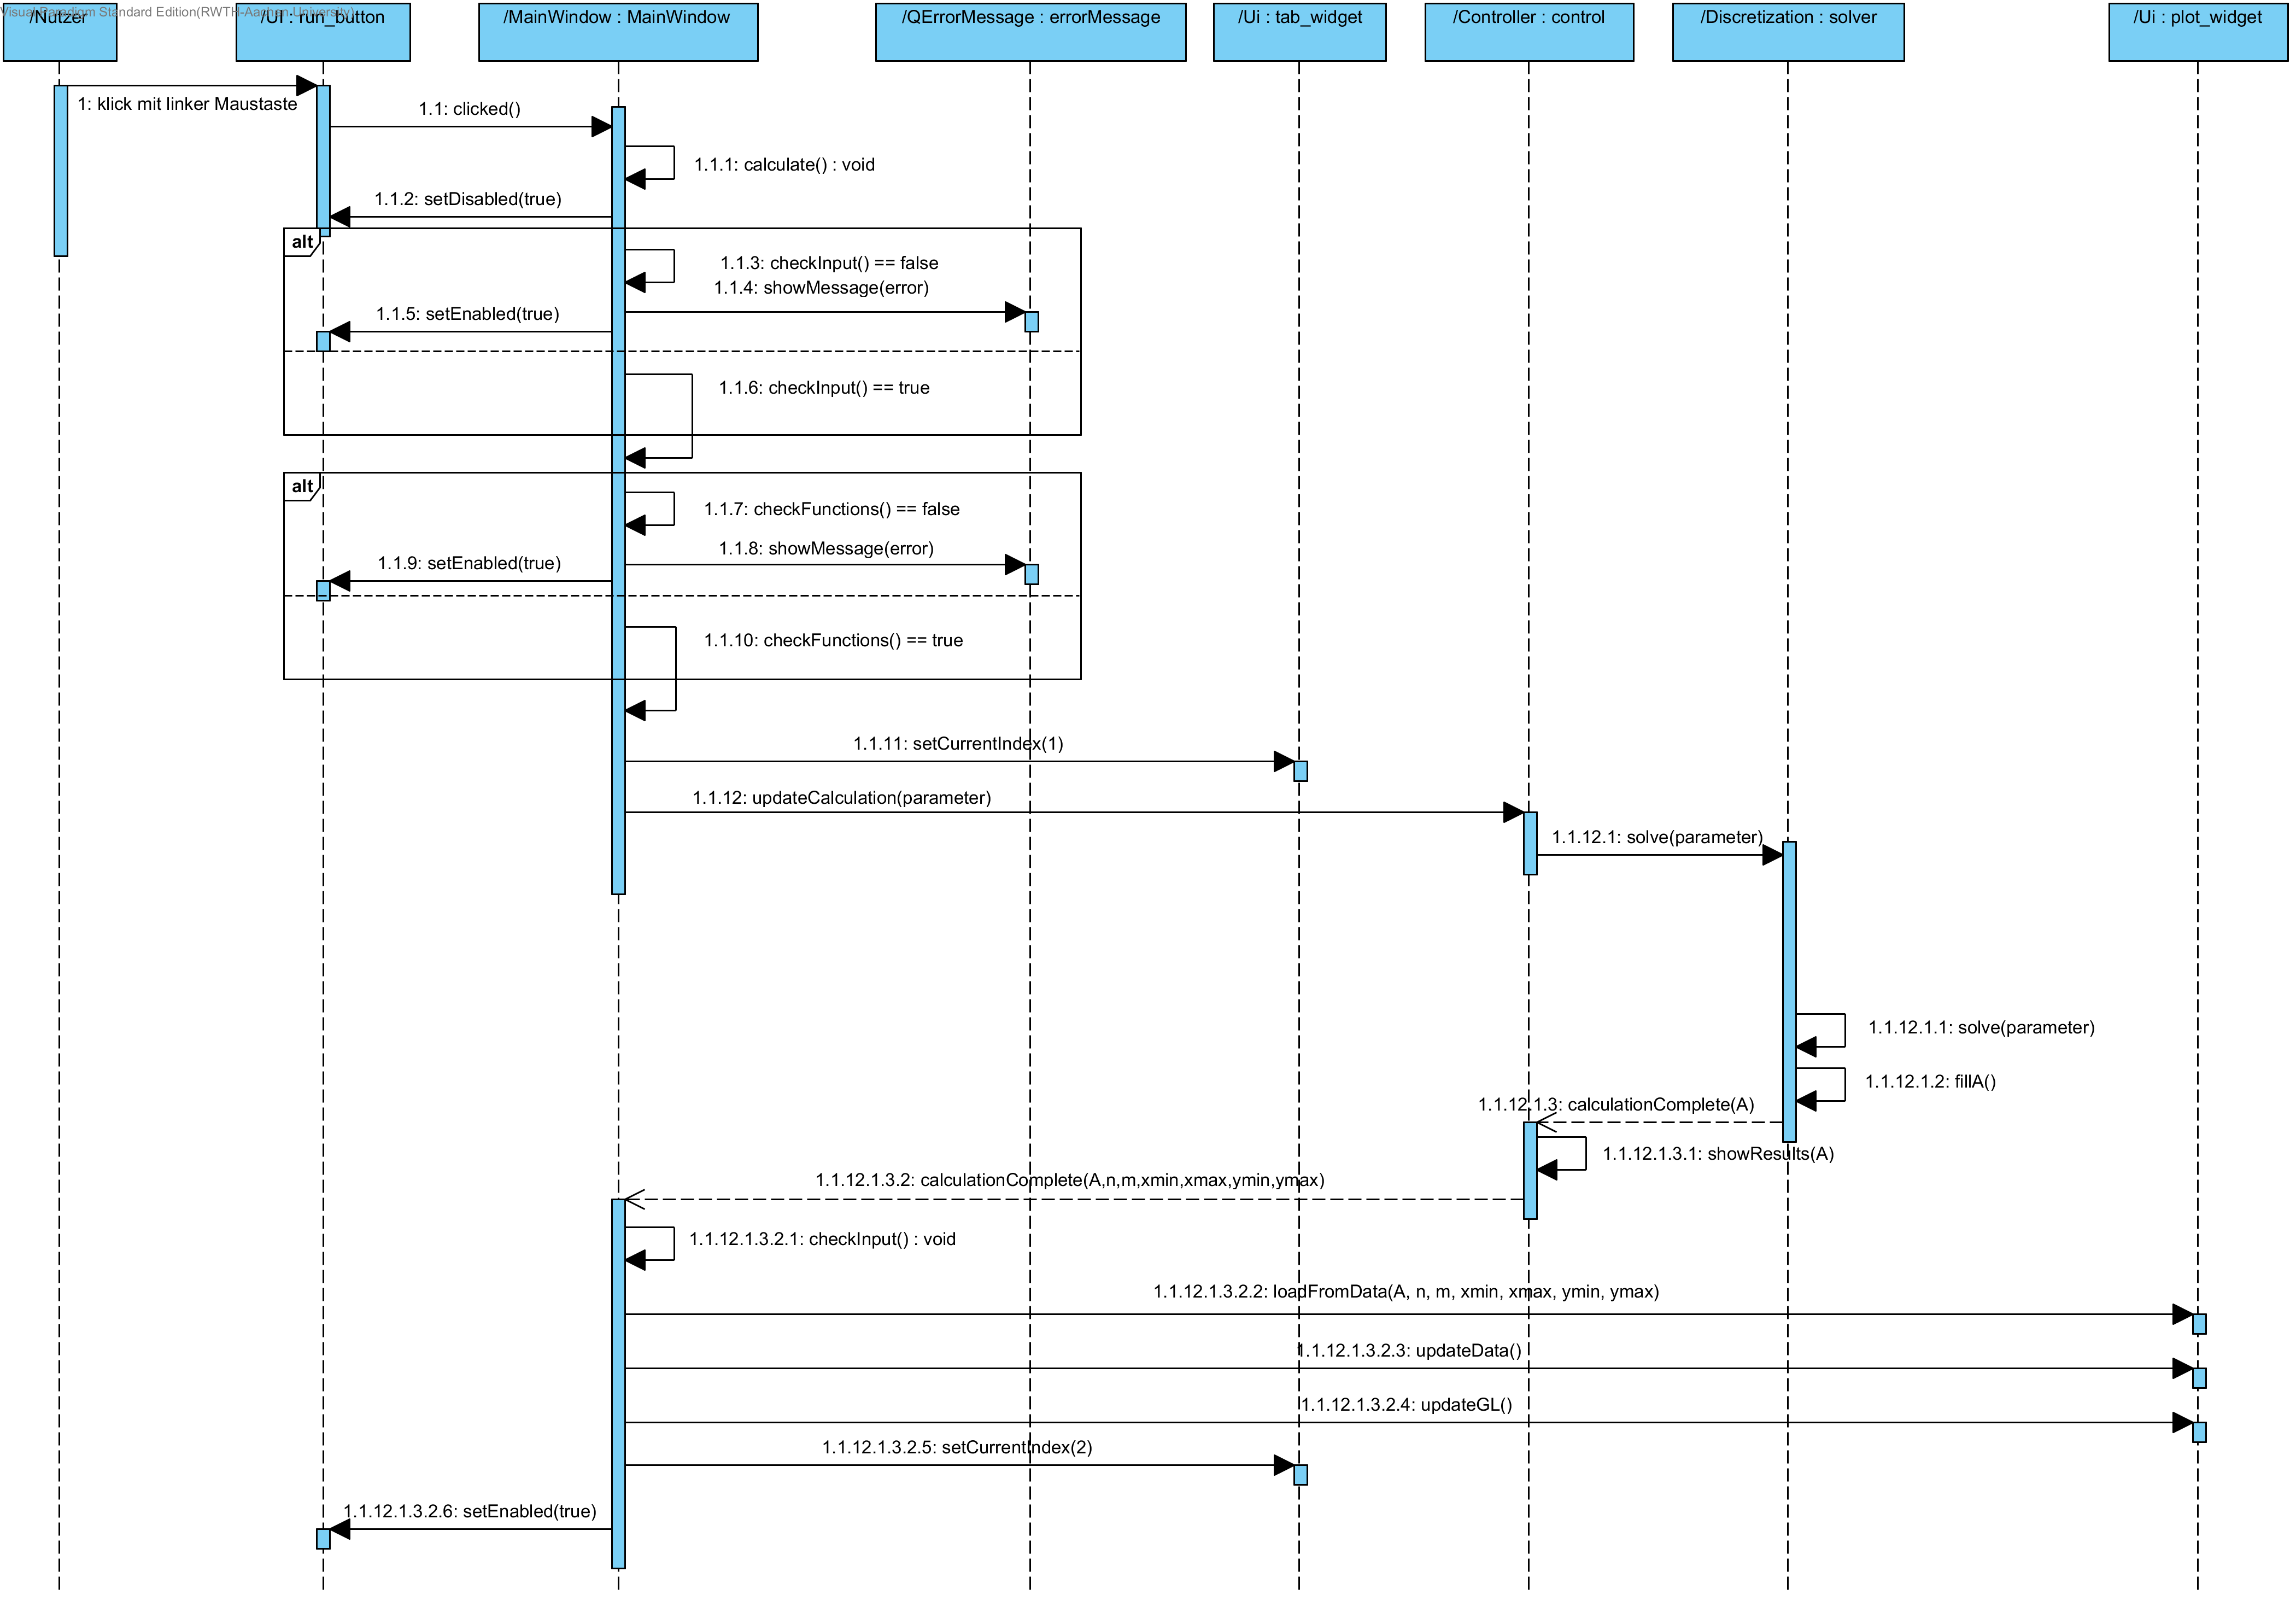
\epsfig{file=Bilder/Run.eps,width=\textwidth}
 \textbf{Tab wechseln} \\ \newline
\epsfig{file=Bilder/Tab_wechseln.eps,width=\textwidth}
\chapter{Benutzerdokumentation}
\label{ch:4}

\section{Installation}
\subsection{Voraussetzungen und Installation der kompilierten Version}
F\"ur die Installation der Software ist ein Linux basiertes Betriebssystem notwendig. Die folgenden Schritte beschreiben den Installationsprozess f\"ur die bereits kompilierte Version. Diese Version wurde auf dem RWTH-Cluster sowie Ubuntu 14.04.3 LTS erfolgreich getestet.
\begin{enumerate}
  \item Entpacken des Archivs {\tt minimalflaechen\_projekt\_gruppe2.zip} in den gew\"unschten Installationsort.
  \item Wechseln in das Verzeichnis {\tt minimalflaechen\_projekt\_build}.
  \item Ausf\"uhren des Skripts {\tt minimalflaechen.sh} \"offnet das Programm. \\ \textit{Hinweis: Um das Skript ausf\"uhren zu k\"onnen m\"ussen gegebenenfalls Rechte f\"ur dieses mithilfe des Befehls {\tt chmod -x ./minimalflaechen.sh} gesetzt werden.}
\end{enumerate}

\subsection{Installation der unkompilierten Version}
Die unkompilierte Version des Programms findet sich in dem Verzeichnis {\tt minimalflaechen\_projekt\_source}. \"Offnen und konfigurieren des Projekts erfordert das Programm Qt Creator sowie die Installation der QT Bibliotheken. Zus\"atzlich dazu m\"ussen die Bibliotheken {\tt qwtplot3d} und {\tt matheval} kompiliert und in die Ordner {\tt libmatheval/lib} und {\tt qwtplot3d/lib} in dem Projektverzeichnis kopiert werden. Der Source-Code der Bibliotheken befindet sich in dem Verzeichnis {\tt ThirdParty}. Die Kompilierung dieser Bibliotheken ist unterschiedlich f\"ur verschiedene Betriebssysteme und erfordert ggf. weitere Bibliotheken. Bei Fragen bitte an {\tt stefan.jeske@rwth-aachen.de} wenden.

{\em wohlstrukturierte und gut lesbare Dokumentation basierend auf
den Anwendungsf\"allen}

\section{Speichern und Laden}
Die Applikation verf\"ugt \"uber eine Speicher- und Lade Funktionalit\"at. Die Einstellungen (Randfunktionen, numerische Parameter und Gebietsgr\"o\ss e) kann man in einem \textbf{.setup} Format und die berechnete Minimalfl\"ache kann man in einem \textbf{.surface} Format speichern und laden
%Evtl ein Bild vom Hauptfenster
\subsection{.setup-Format}
Das Speichern und Laden der Einstellungen arbeiten mit Dateien im \textbf{.setup}-Format.
Die Datei ist so aufgebaut, dass sich in jeder Zeile Informationen zu den eingegebenen Werten/Funktionen befinden, welche mit einem Semikolon am Ende abgetrennt werden. 
Dabei spielt die Reihenfolge der Informationen eine wichtige Rolle. Die Informationen von der ersten bis zur letzten Zeile:
\begin{enumerate}
\item epsilon - Genauigkeit der L\"osung
\item iterations - Maximale Iterationsschritte
\item n - Anzahl der St\"utzstellen in x-Richtung
\item m - Anzahl der St\"utzstellen in y-Richtung
\item xmin - untere x-Grenze
\item xmax - obere x-Grenze
\item ymin - untere y-Grenze
\item ymax - obere y-Grenze
\item a - Randfunktion auf der linken Seite des Gebietes
\item b - Randfunktion auf der oberen Seite des Gebietes
\item c - Randfunktion auf der rechten Seite des Gebietes
\item d - Randfunktion auf der unteren Seite des Gebietes
\end{enumerate}
%Bild Einstellungen_Speichern_2.png
\hfill \newline
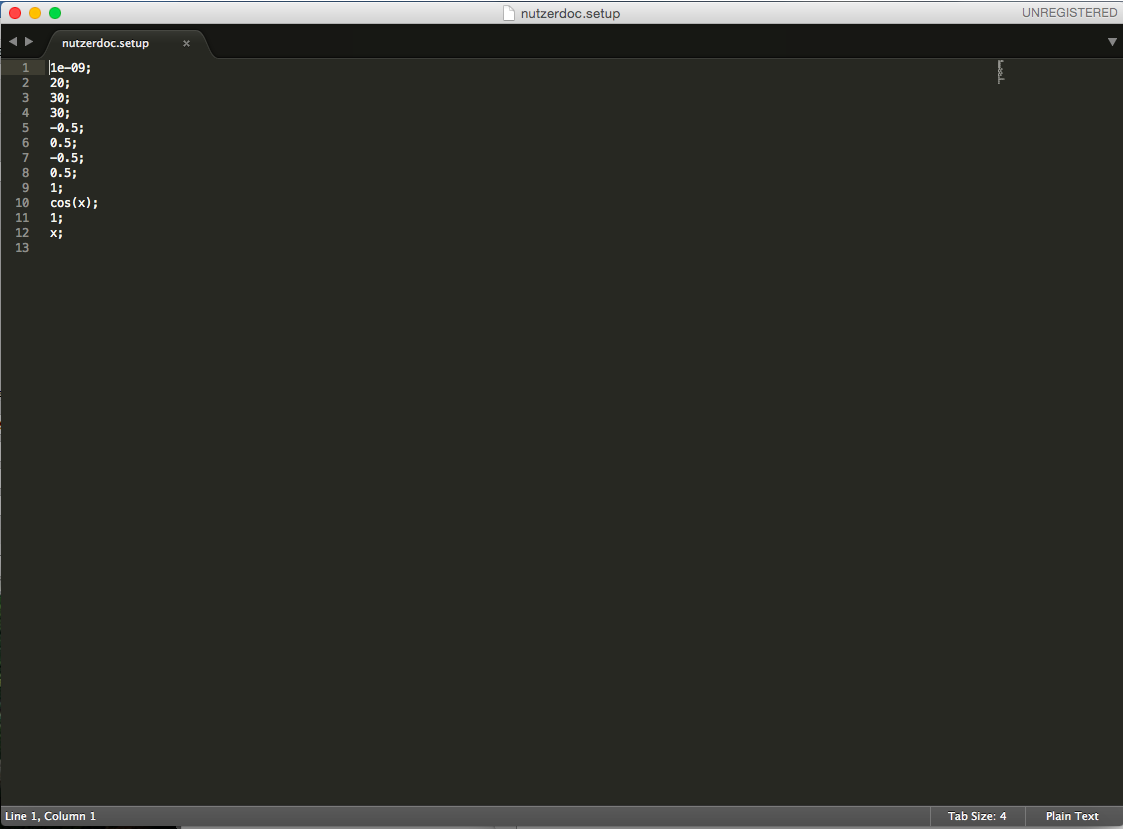
\epsfig{file=nutzerdoc/Einstellung_Speichern_2.eps,width=\textwidth}
\subsection{.surface-Format}
Das Speichern und Laden der Einstellungen arbeiten mit Dateien im \textbf{.surface}-Format
Eine \textbf{.surface}-Datei ist in zwei Abschnitten aufgebaut. 
Im ersten Abschnitt enth\"alt die Datei ein paar grundlegende Informationen zu den Eingabedaten der Berechnung:
\begin{enumerate}
\item n - Anzahl der St\"utzstellen in x-Richtung
\item m - Anzahl der St\"utzstellen in y-Richtung
\item iterations - Maximale Iterationsschritte
\item epsilon - Genauigkeit der L\"osung
\item xmin - untere x-Grenze
\item xmax - obere x-Grenze
\item ymin - untere y-Grenze
\item ymax - obere y-Grenze
\end{enumerate}
Der zweite Abschnitt enth\"alt die berechnete Minimalfl\"ache inklusive den ausgewerteten R\"andern.
Jeder Wert wird mit einem Semikolon getrennt und insgesamt stellen die Zahlen die Eintr\"age von der Ergebnismatrix dar. (L\"osung von Ax=b, mit x als eine Matrix transformiert)

Hinweis: Die L\"osung der Minimalfl\"ache ist so gespeichert, dass man die Daten mit Programmen wie Excel oder Matlab weiterarbeiten kann. Die Semikolons dienen zur Trennung zwischen den einzelnen Daten, wie sie bei Excel z.B. mit unterschiedlichen Zellen realisiert werden.

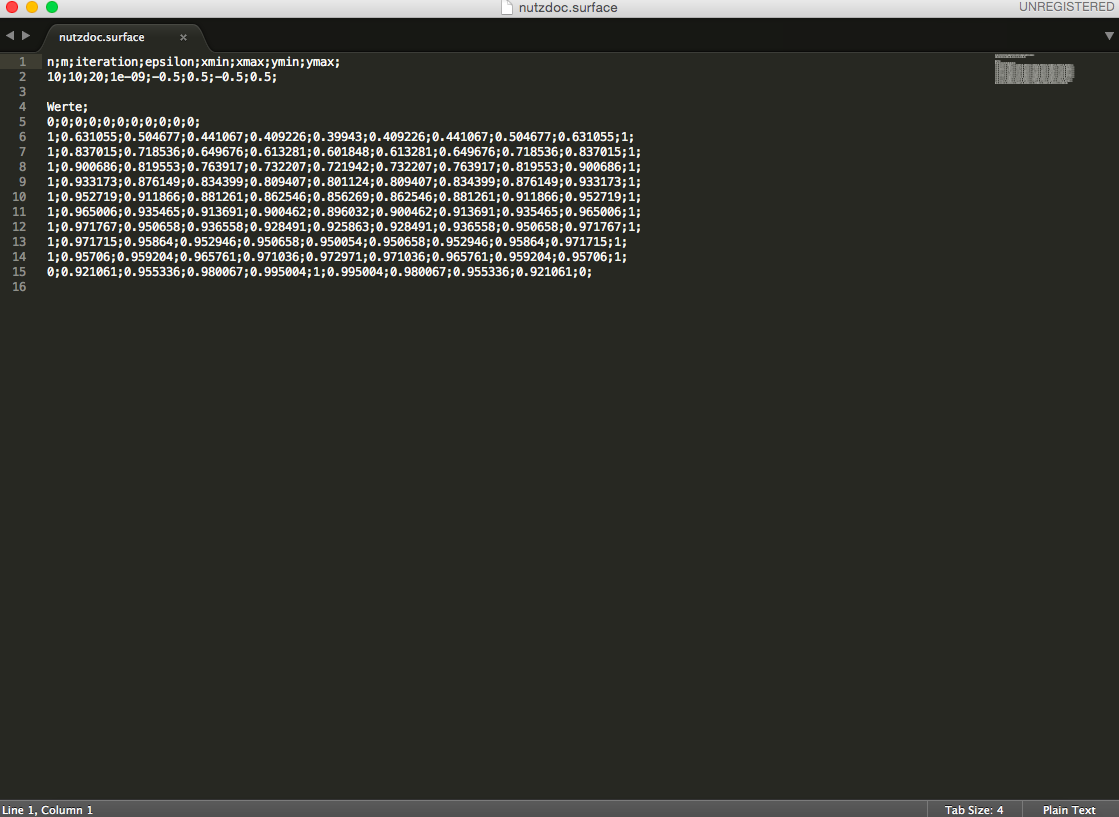
\epsfig{file=nutzerdoc/surface_format.eps,width=\textwidth}

Nachdem der Nutzer den Button "'Einstellungen speichern" geklickt hat, erscheint ein Dialogfenster, wo der Nutzer den Speicherpfad, sowie den Dateinamen eingeben kann. Nach der Bet\"atigung des Save Buttons wird dann die Datei im \textbf{filename.setup} erstellt. 
\newline
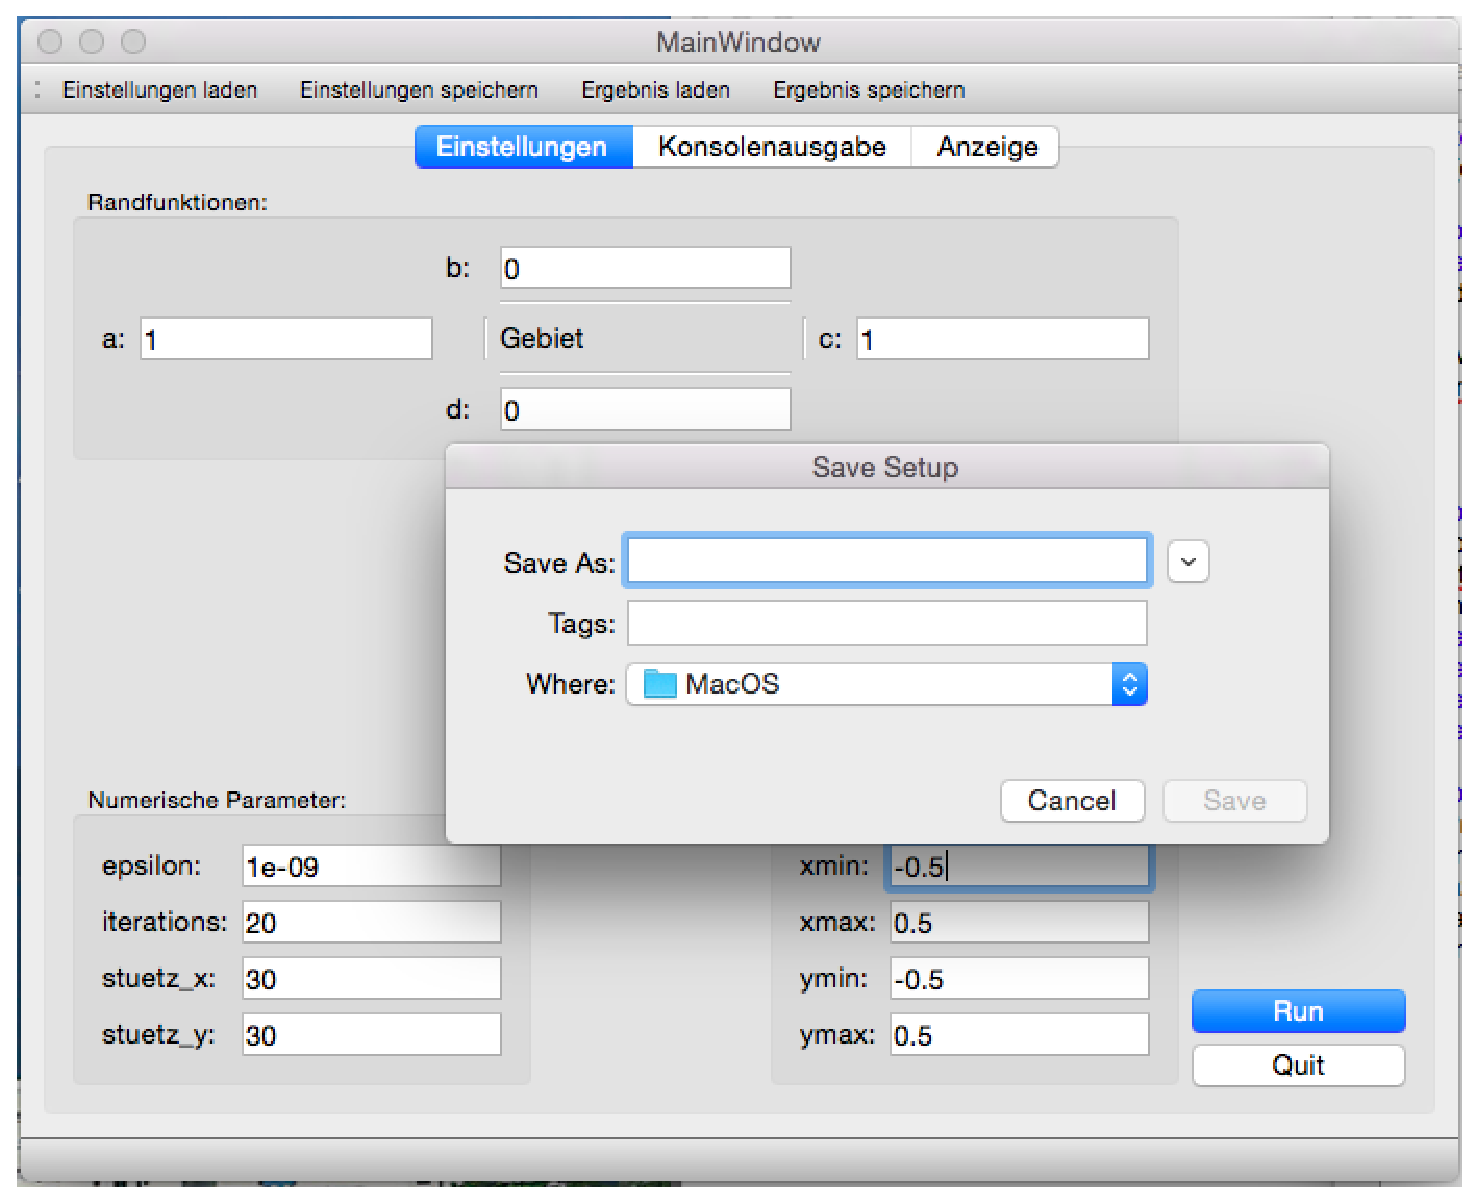
\epsfig{file=nutzerdoc/Einstellung_Speichern_1.eps,width=\textwidth}
% Bild Einstellungen_Speichern_1.png

\subsection{Einstellungen laden}
Nachdem der Nutzer den Button "'Einstellungen laden" geklickt hat, erscheint ein Dialogfenster, wo der Nutzer das Verzeichnis suchen kann, wo sich die Datei im \textbf{.setup}-Format befindet. Durch anschlie\ss endes Klicken auf den Open-Button werden die Randfunktionen, numerischen Parameter sowie die Gebietsgr\"o\ss e im Tab Einstellungen aktualisiert.
\newline
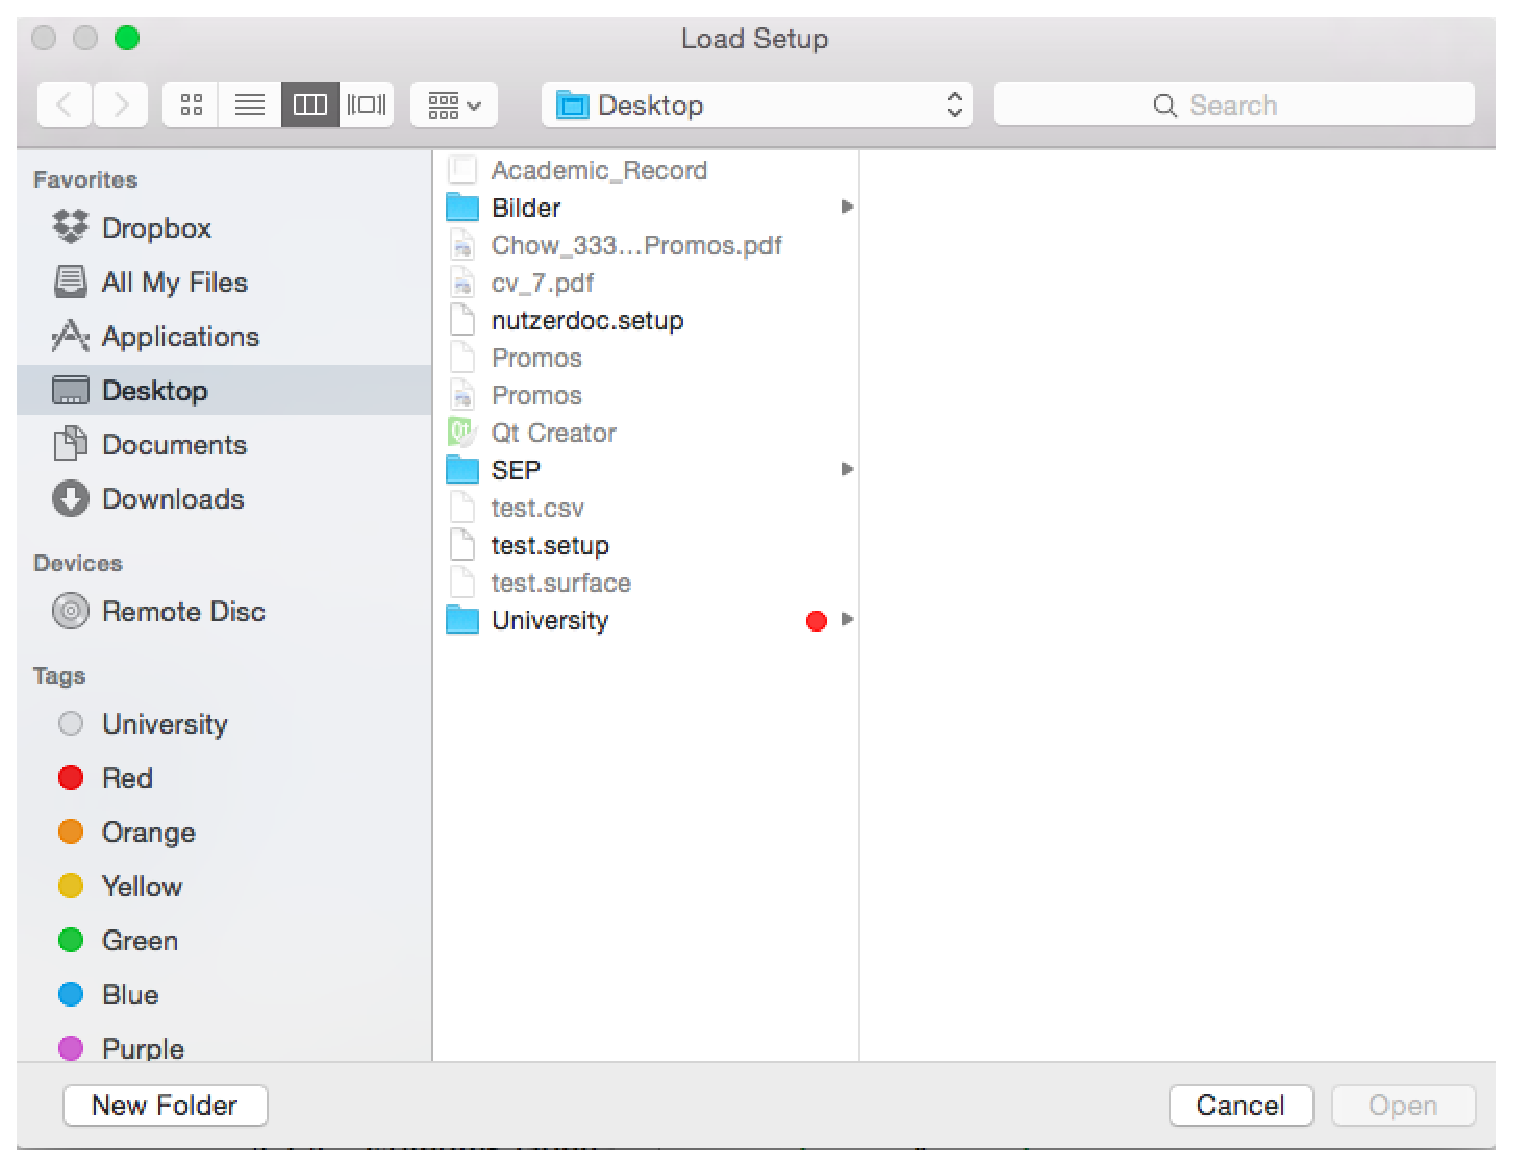
\epsfig{file=nutzerdoc/Einstellung_Laden_1.eps,width=\textwidth}

%Bild Einstellung_Laden_1.png
\subsection{Ergebnis speichern}
Nachdem der Nutzer den Button "'Ergebnis speichern" geklickt hat, erscheint ein Dialogfenster, wo der Nutzer den Speicherpfad, sowie den Dateinamen eingeben kann. Nach der Bet\"atigung des Savebuttons wird dann die Datei im \textbf{filename.surface} erstellt.
Hinweis: Speicherung eines Ergebnisses erst nach der Berechnung m\"oglich.
\newline
\epsfig{file=nutzerdoc/Ergebnis_Speichern.eps,width=\textwidth}
% Bild Ergebnis_Speichiern.png
\subsection{Ergebnis laden}
Nachdem der Nutzer den Button "'Ergebnis laden" geklickt hat, erscheint ein Dialogfenster, wo der Nutzer das Verzeichnis suchen kann, wo sich die Datei im \textbf{.surface}-Format befinet. Durch anschlie\ss endes Klicken auf den Open-Button werden die Ergebnisse geladen und die Minimalfl\"ache angezeigt. \newline
% Bild Ergebnis_Laden.png 
\epsfig{file=nutzerdoc/Ergebnis_Laden.eps,width=\textwidth}

\subsection{Mit der .surface-Datei weiterarbeiten}
In diesem Abschnitt wird eine kurz Einf\"uhrung gegeben, wie man mit einer .surface-Datei in  \"ublichen Datenanalyseprogrammen weiterarbeiten kann. Als Beispiel wird hierf\"ur \textbf{MATLAB} genommen. \\
%% Bild Matlaboberfl�che
\epsfig{file=nutzerdoc/3.eps,width=\textwidth}
\\ 
Nachdem man auf \textit{Import Data} geklickt hat, muss man bei den Dateientypen \textbf{All files} ausw\"ahlen, damit die .surface-Dateien zur Auswahl angezeigt werden kann. In unserem Fall importieren wir die Daten aus der Datei \textit{standard.surface}. Nachdem man die zu ausgewerteten Daten markiert hat und die Importeinstellung \textit{Numeric Matrix} ausgew\"ahlt ist, kann man unter \textit{Import Selection} die Unterfunktion \textit{Generate Script} anklicken.
\\
\epsfig{file=nutzerdoc/1.eps,width=\textwidth}
\\
Nun werden die Daten in Matlab geladen, welche z.B. mit dem Befehl \textbf{surf(filename)} geplottet werden k\"onnen.
\\
\epsfig{file=nutzerdoc/tier1.eps,width=\textwidth}
\\
\section{Eingaben}
Das Programm besitzt zwar eingebaute Erkennung richtiger Eingabewerte, jedoch nicht Erkennung sinnvoller Eingabewerte, d.h. wie sich die Rechenzeit in Abh\"angigkeit der eingegebenen Parameter verh\"alt. Im Folgenden sind also Wertebereiche beschrieben, bei denen das Programm nicht l\"anger als eine Minute Laufzeit auf einem durchschnittlichen Laptop hatte. 
\begin{itemize}
  \item $ \epsilon \in [10^{-9},1] $
  \item $ iterations \in [10,20] $
  \item $ stuetz_x, stuetz_y \in [10,60] $
\end{itemize}
Am gr\"o\ss ten beeinflusst wird die Laufzeit des Programms durch die gew\"ahlte Anzahl der St\"utzstellen. \\
Die Wahl der Randfunktionen ist relativ beliebig und gut gesch\"utzt, d.h. durch Fehlersituationen abgefangen. Ebenso beliebig ist die Wahl des Definitionsbereichs, welche auch durch entsprechende Fehlermeldungen gesch\"utzt ist. \\
Weiterhin werden die Randfunktionen nur auf ihre Syntaktische Korrektheit �berpr�ft und nicht auf m\"ogliche Singularit\"aten oder Divisionen durch Null. Dies kann ein Grund f\"ur Divergenz des L\"osers sein.
Deshalb sollte beachtet werden, dass keine Kovergenz, bzw. kein sinnvolles Ergebnis, f�r das vom Benutzer gestellten Problems garantiert wird.

\section{Beispielsitzung}
Nun wird eine Beispielsitzung in dem Programm durchgef\"uhrt. In der Sitzung werden zwei Berechnungen ausgef\"uhrt, Einstellungen geladen und Ergebnisse gespeichert.
Zun\"achst jedoch wird das Programm gestartet.

\begin{figure}[H]
\centering
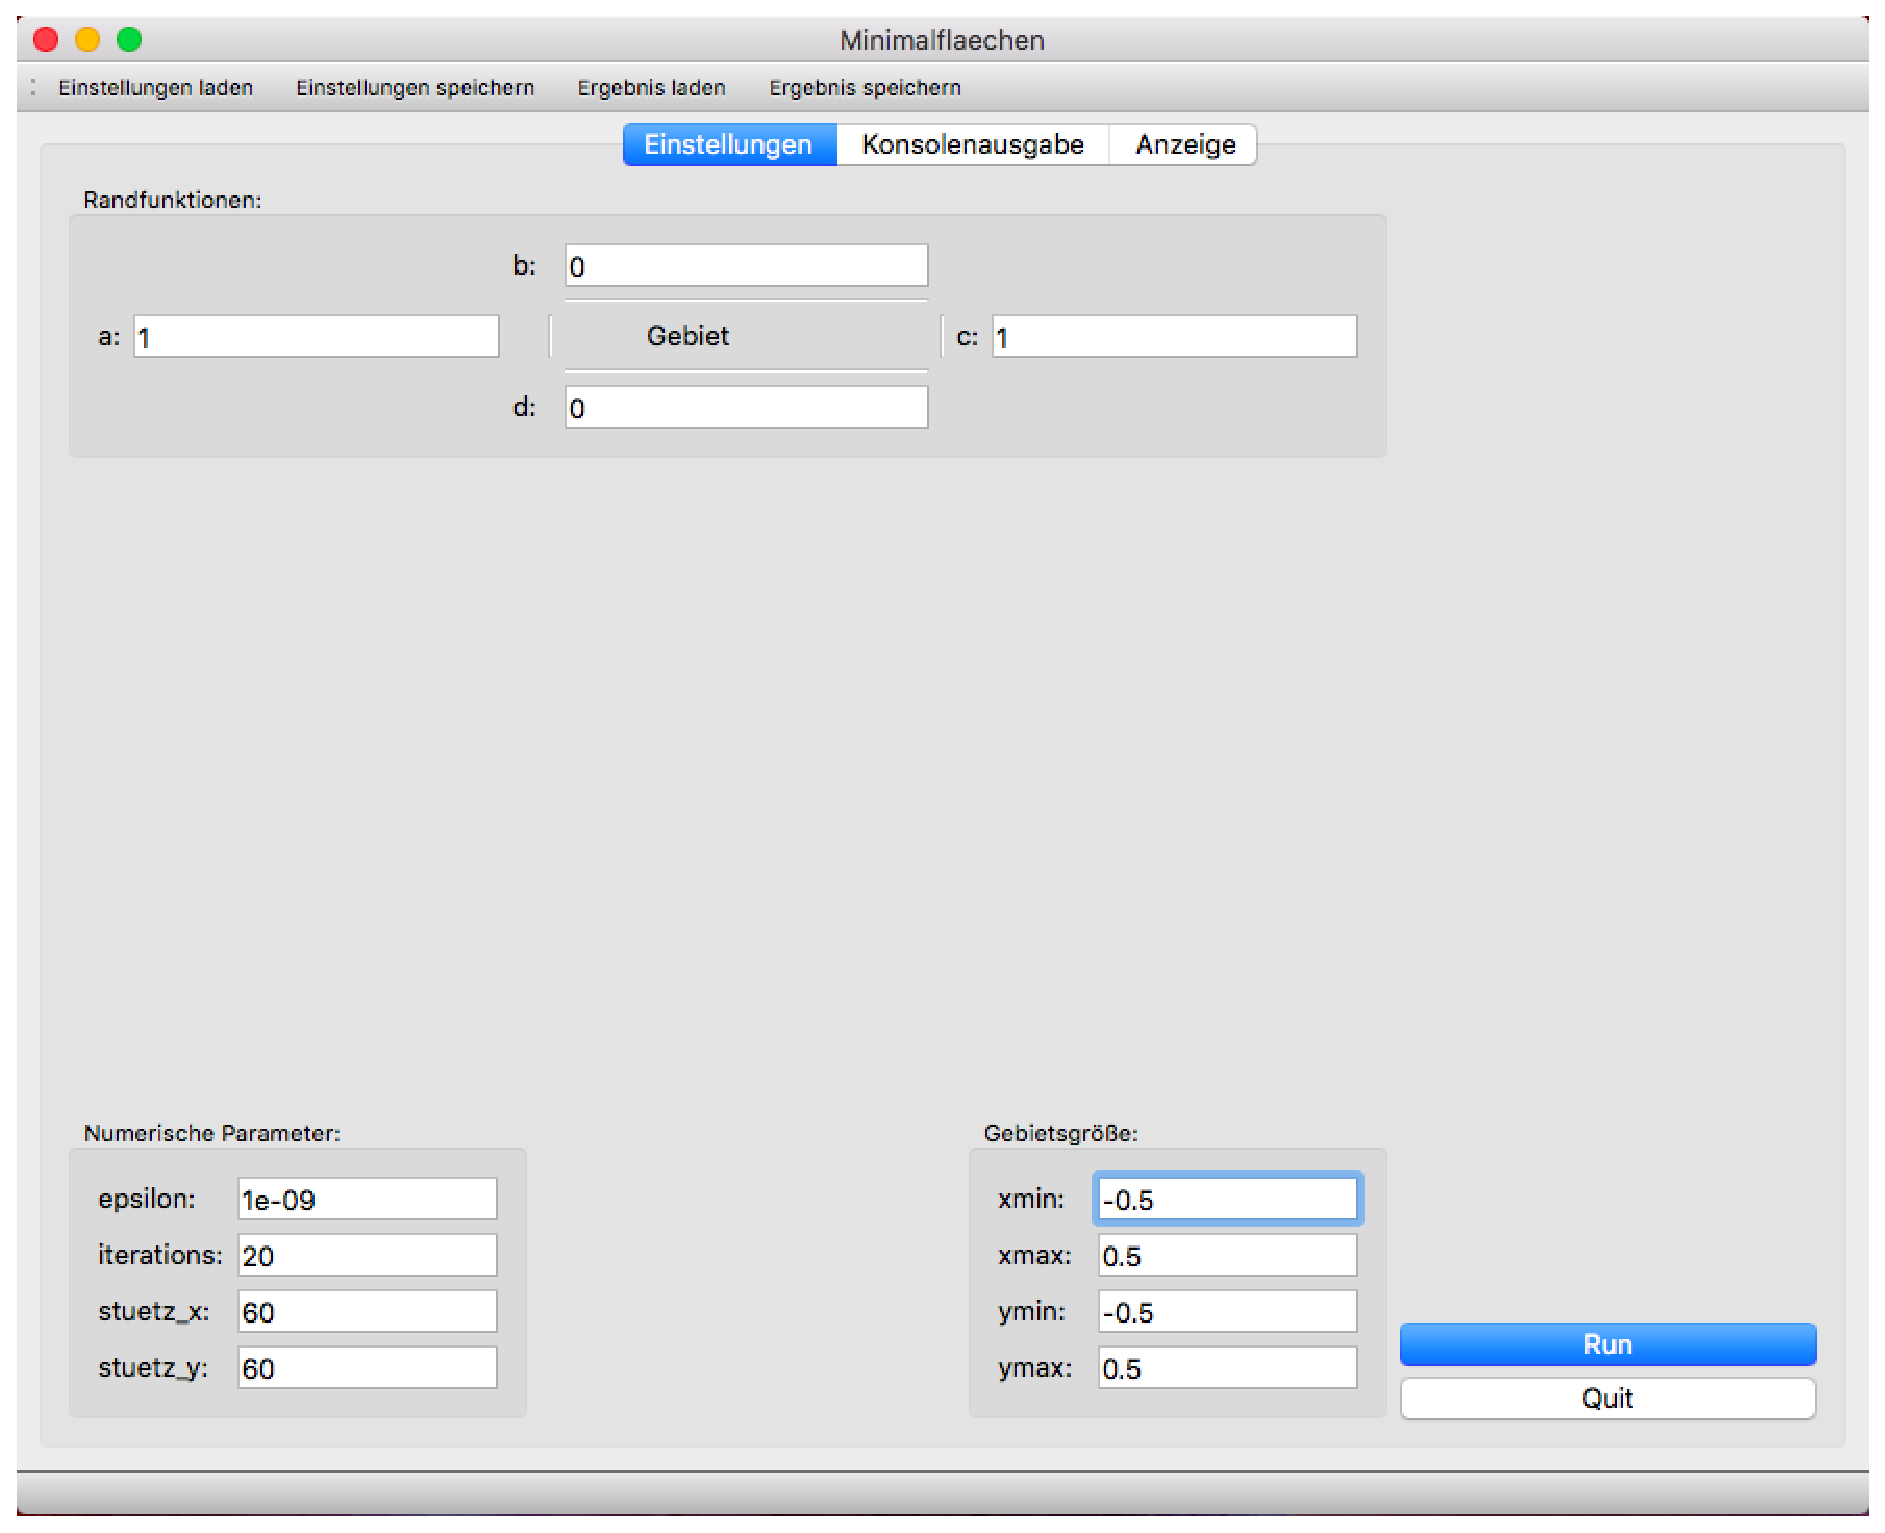
\includegraphics[width=\textwidth]{nutzerdoc/example_session/bsp_1}
\caption{Startbildschirm des Programms}
\end{figure}

In dem Startbildschirm k\"onnen alle relevanten Einstellungen f\"ur die Berechnung der Minimalfl\"ache festgelegt werden. In diesem Beispiel wird jedoch direkt auf den {\tt run} Button geklickt. Dies wechselt die Ansicht auf den mittleren Tab {\tt Konsolenausgabe}.

\begin{figure}[H]
\centering
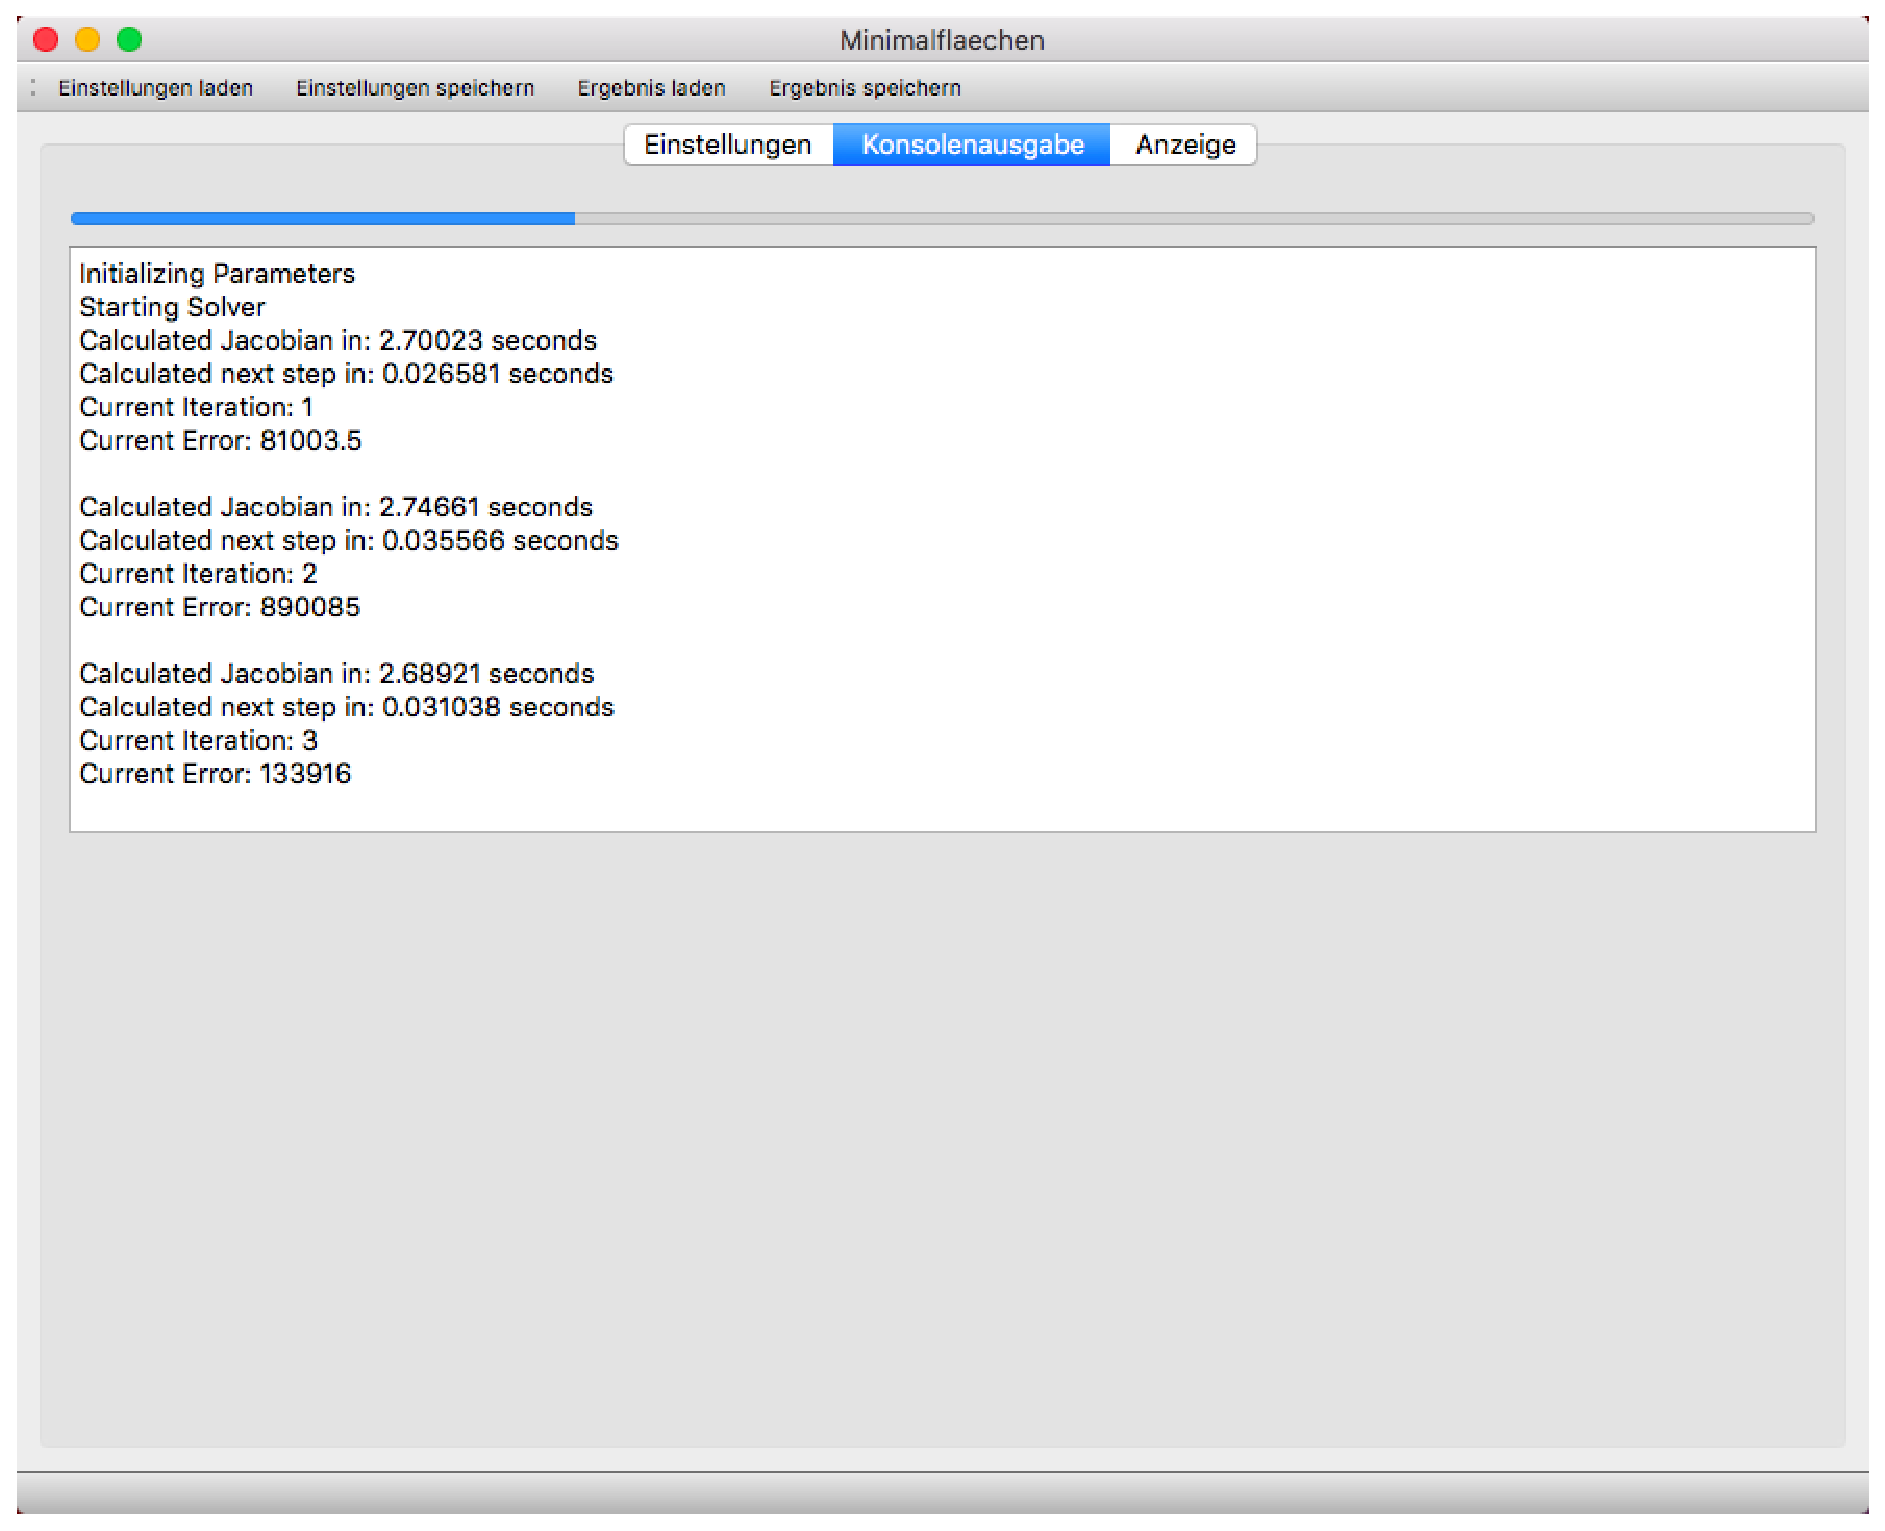
\includegraphics[width=\textwidth]{nutzerdoc/example_session/bsp_2}
\caption{Startbildschirm des Programms}
\end{figure}

Hier ist der aktuelle Berechnungsfortschritt zu sehen, sowie der Konvergenzfehler und ben\"otigte Zeit der einzelnen Iterationen. Am Ende der Berechnung ist hier auch zu sehen, ob die Problemstellung zu dem gew\"unschten Fehler konvergiert ist. Nun wird auf den {\tt Anzeige} Tab gewechselt. 

\begin{figure}[H]
\centering
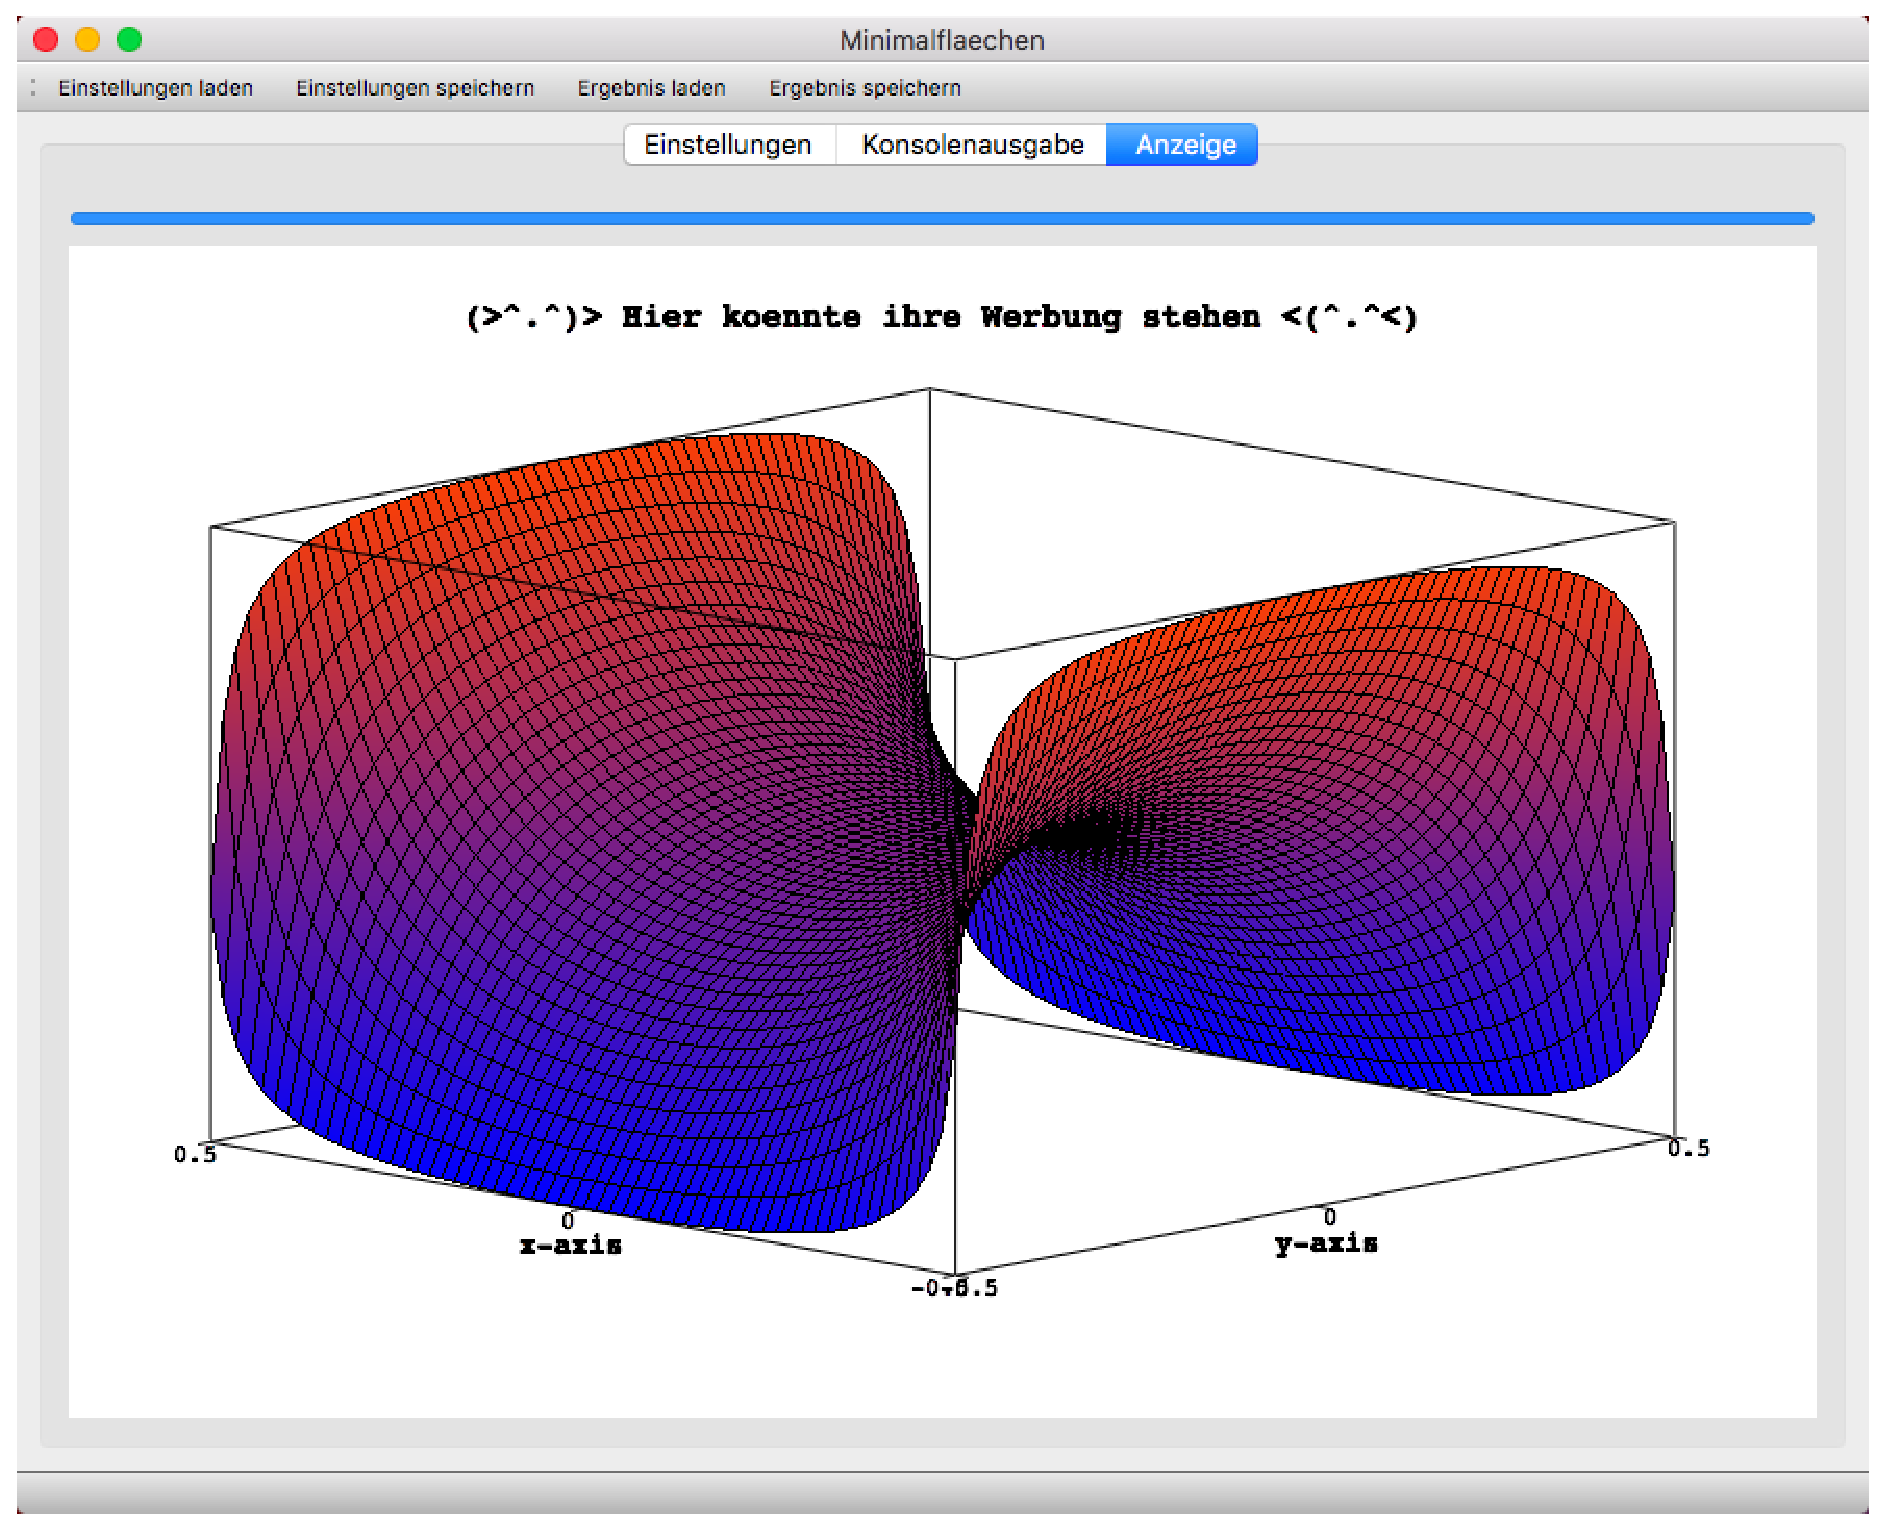
\includegraphics[width=\textwidth]{nutzerdoc/example_session/bsp_3}
\caption{Startbildschirm des Programms}
\end{figure}

Hier wird das Ergebnis der Berechnung angezeigt. Es kann ganz intuitiv in das Ergebnis geklickt werden, um die Fl\"ache z.B. zu Rotieren oder Skalieren. Da dieses Ergebnis keine wirkliche Relevanz hat, wird es dieses Mal nicht gespeichert. Anstelle dessen werden die Einstellung des Referenzproblems geladen.

\begin{figure}[H]
\centering
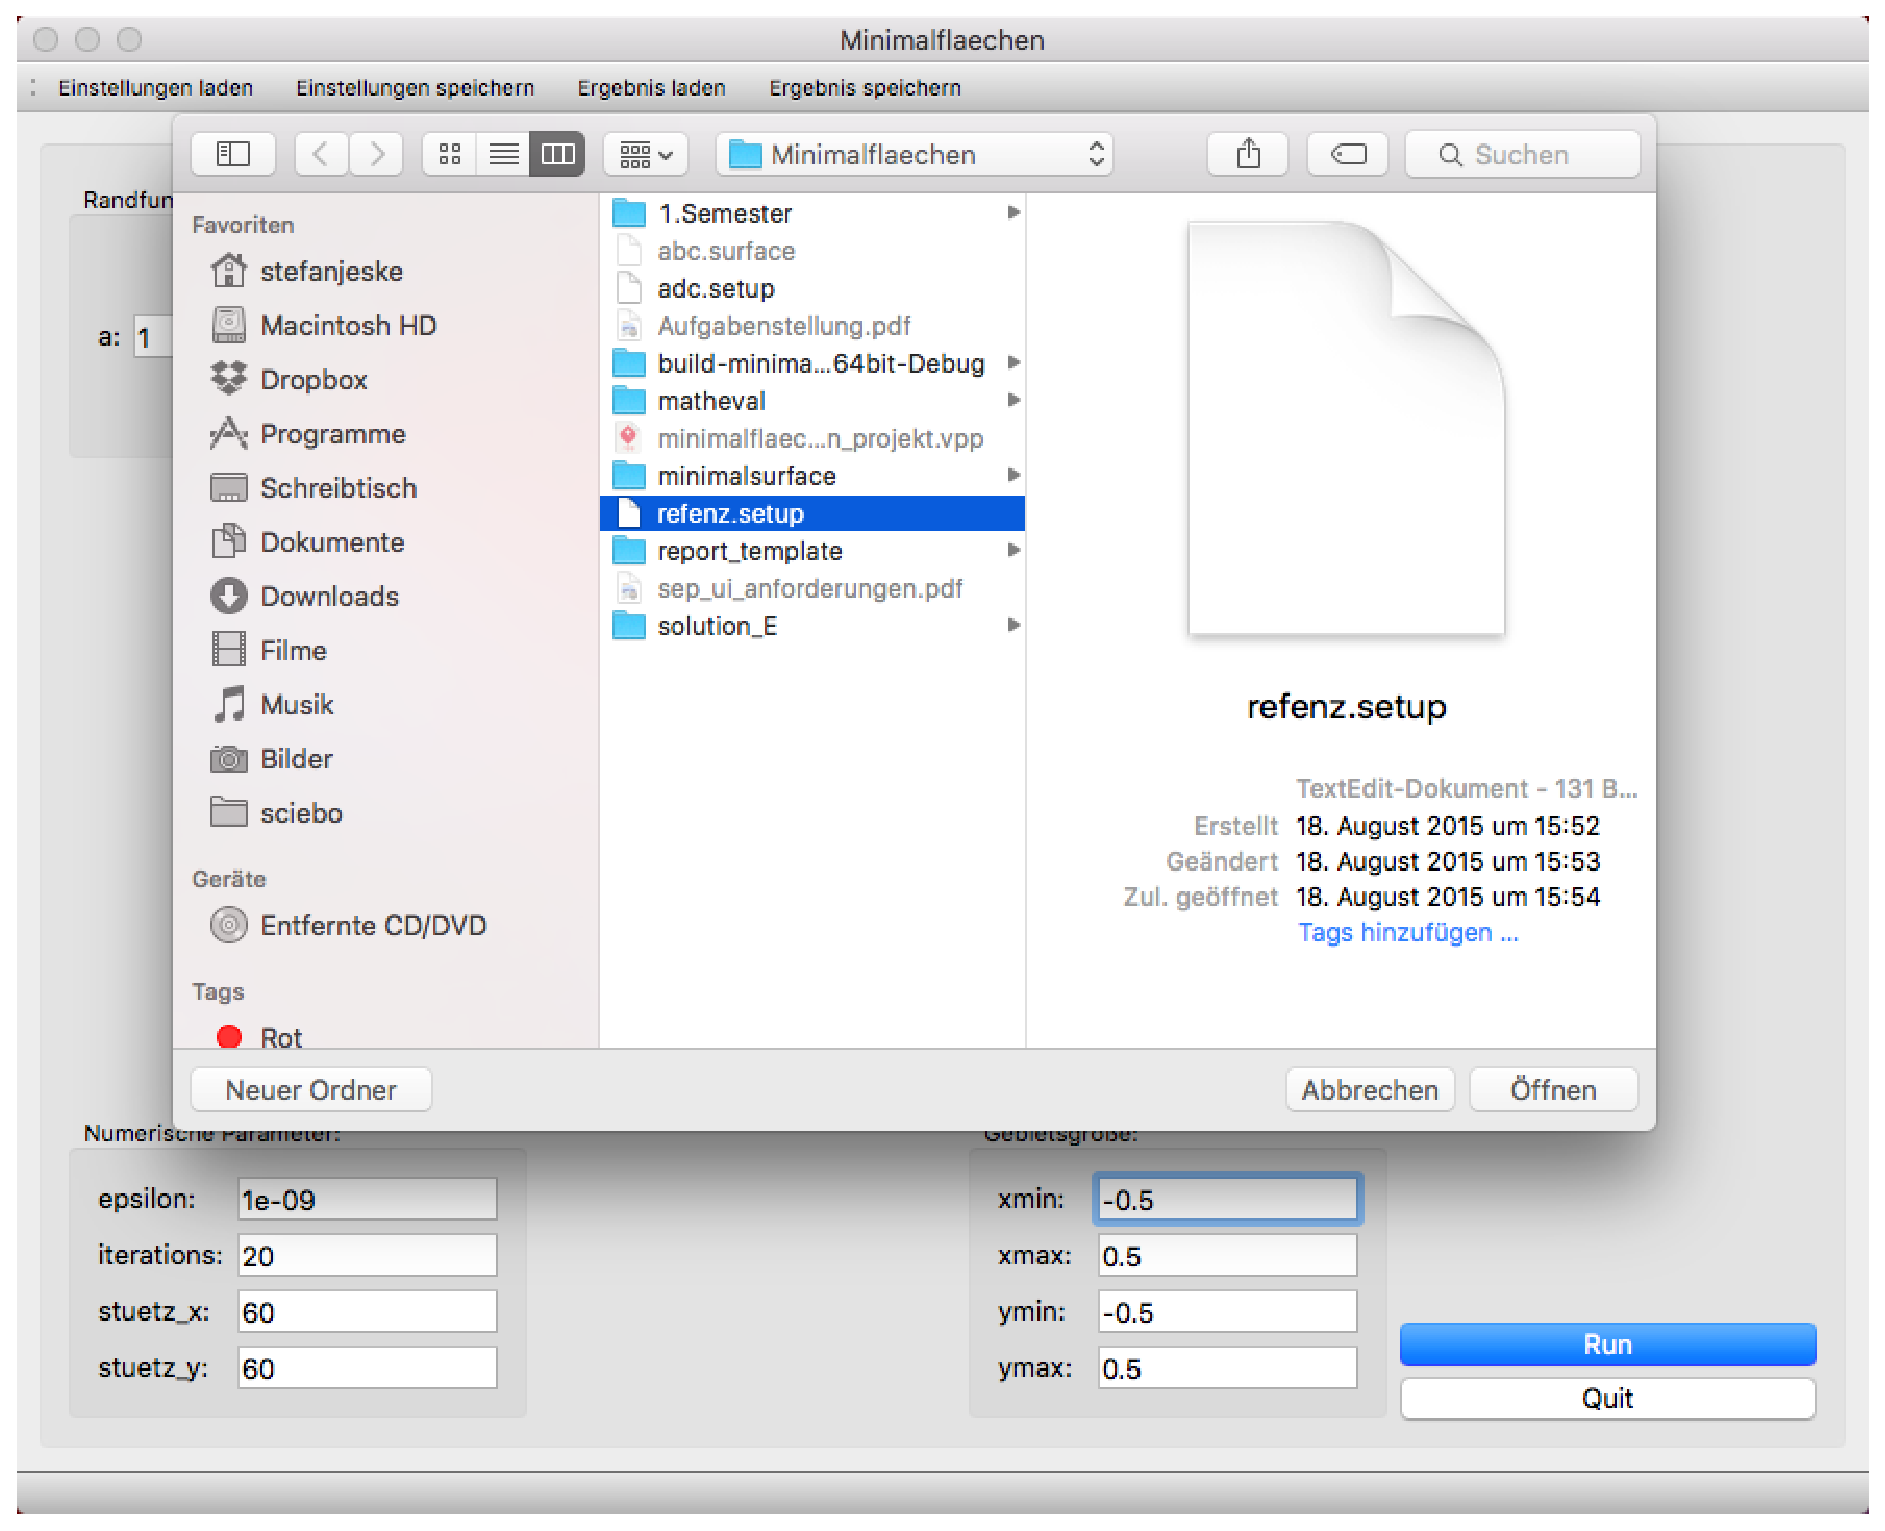
\includegraphics[width=\textwidth]{nutzerdoc/example_session/bsp_4}
\caption{Startbildschirm des Programms}
\end{figure}

Dazu wird auf die Schaltfl\"ache {\tt Einstellungen laden} geklickt und die Datei {\tt referenz.setup} ausgew\"ahlt. Anschlie\ss end wird auf \"offnen geklickt, wodurch die Einstellungen in das Programm geladen werden.

\begin{figure}[H]
\centering
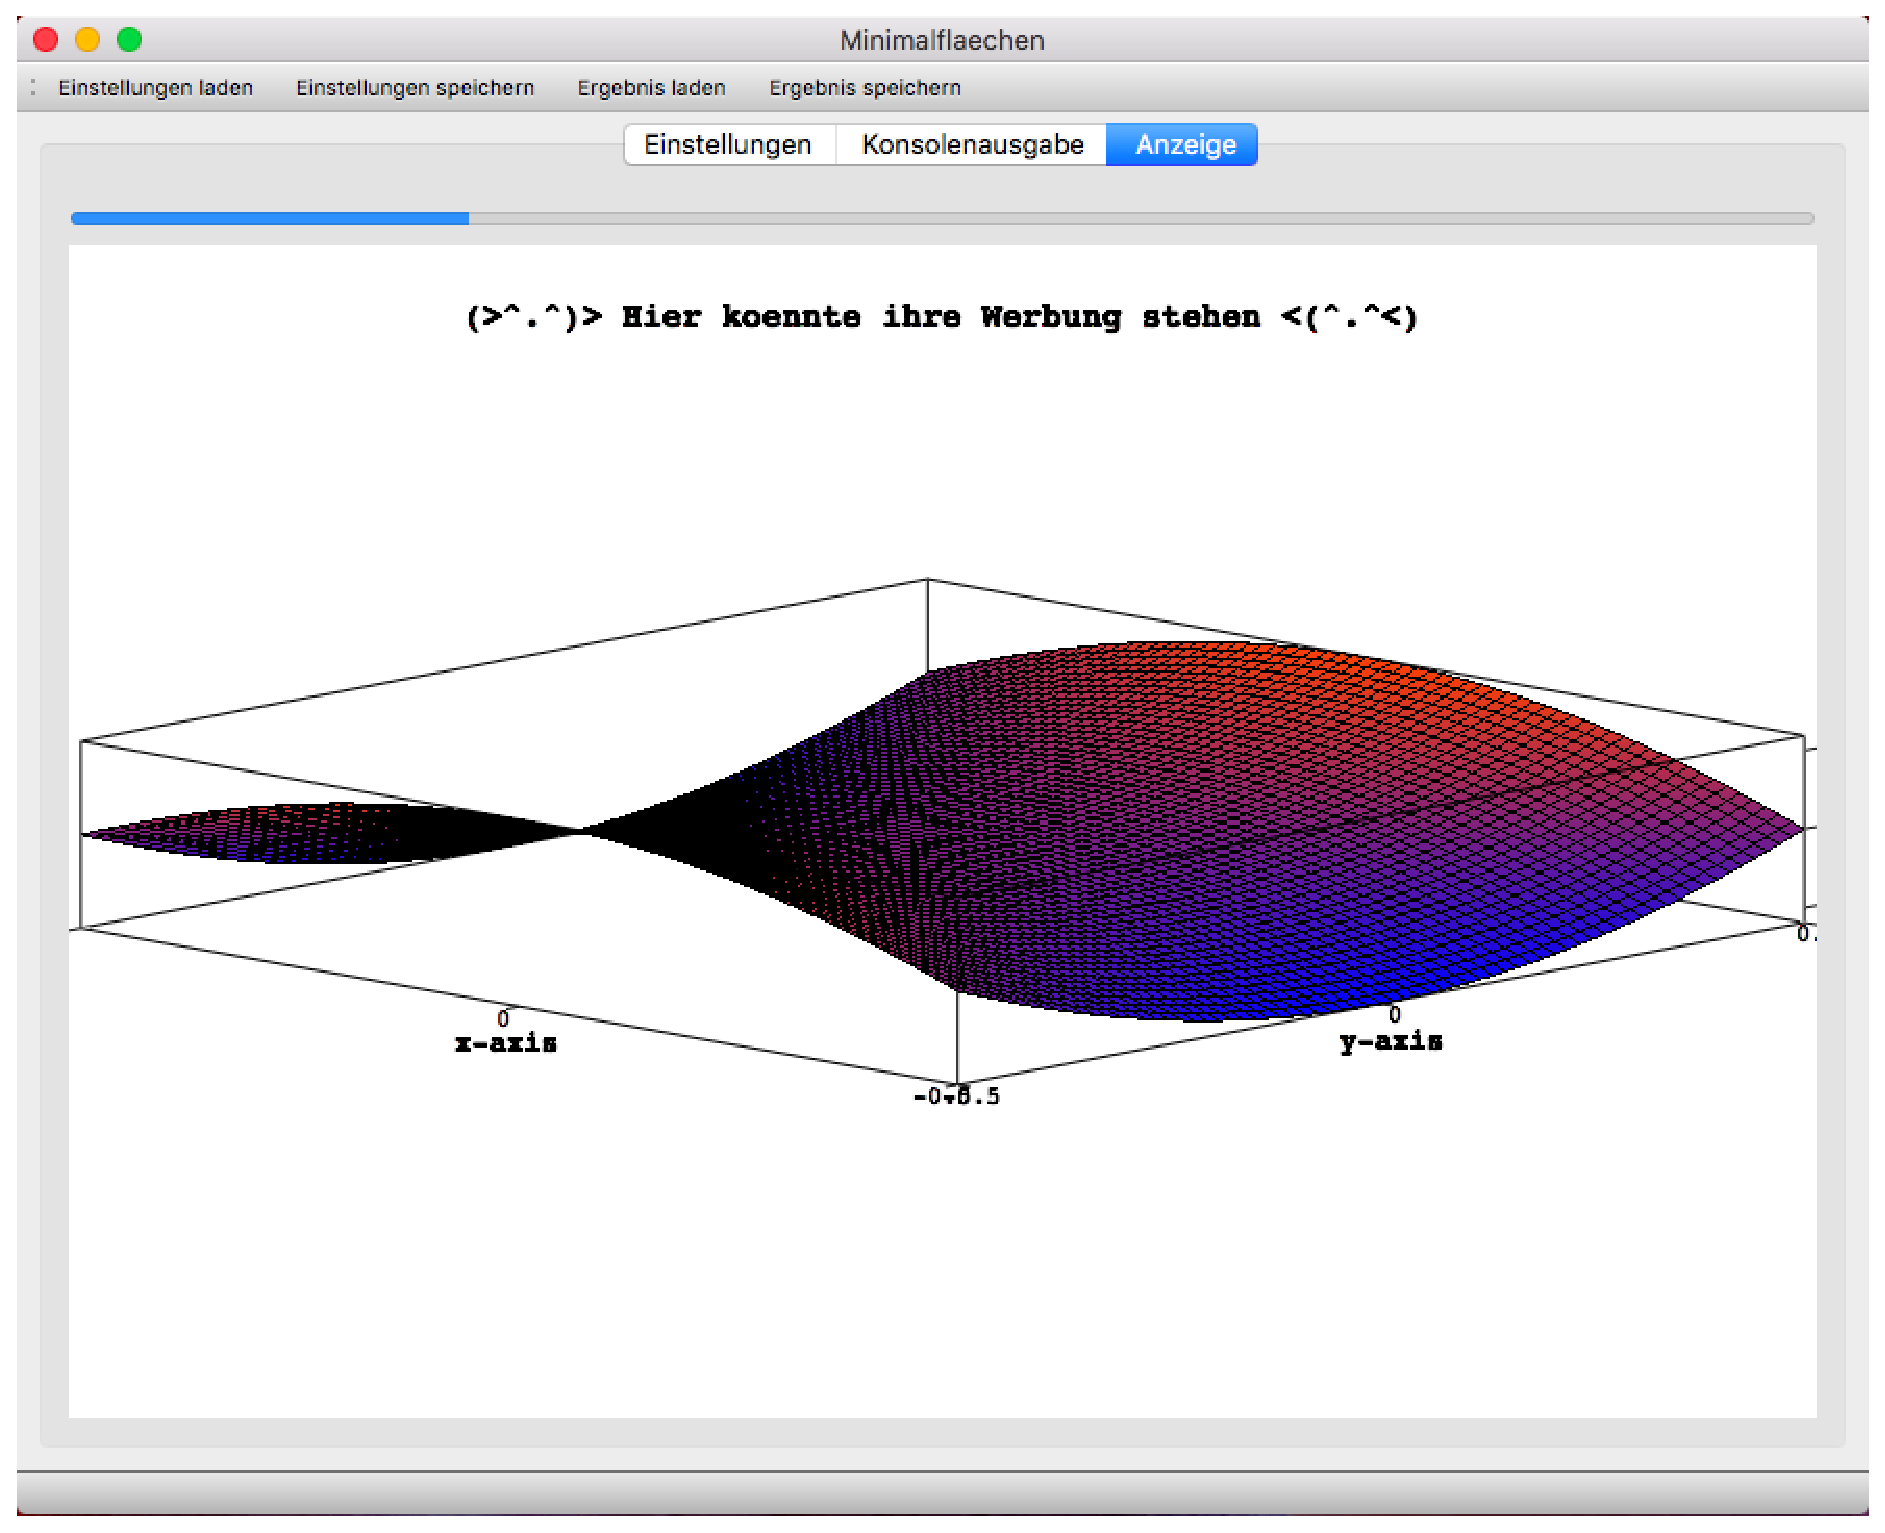
\includegraphics[width=\textwidth]{nutzerdoc/example_session/bsp_5}
\caption{Startbildschirm des Programms}
\end{figure}

Erneut wird auf den {\tt Run} Button geklickt, sodass die Berechnung gestartet wird. Jedoch anstelle wird direkt auf den Tab {\tt Anzeige} gewechselt, um die Entwicklung der Minimalfl\"ache in Echtzeit mitzuvervolgen. Wenn der Fortschrittsbalken voll ist, ist die Berechnung fertig. F\"ur Konvergenz und Rechenzeit kann der {\tt Konsolenausgabe} Tab ge\"offnet werden. Nun wollen wir dieses Ergebnis speichern.

\begin{figure}[H]
\centering
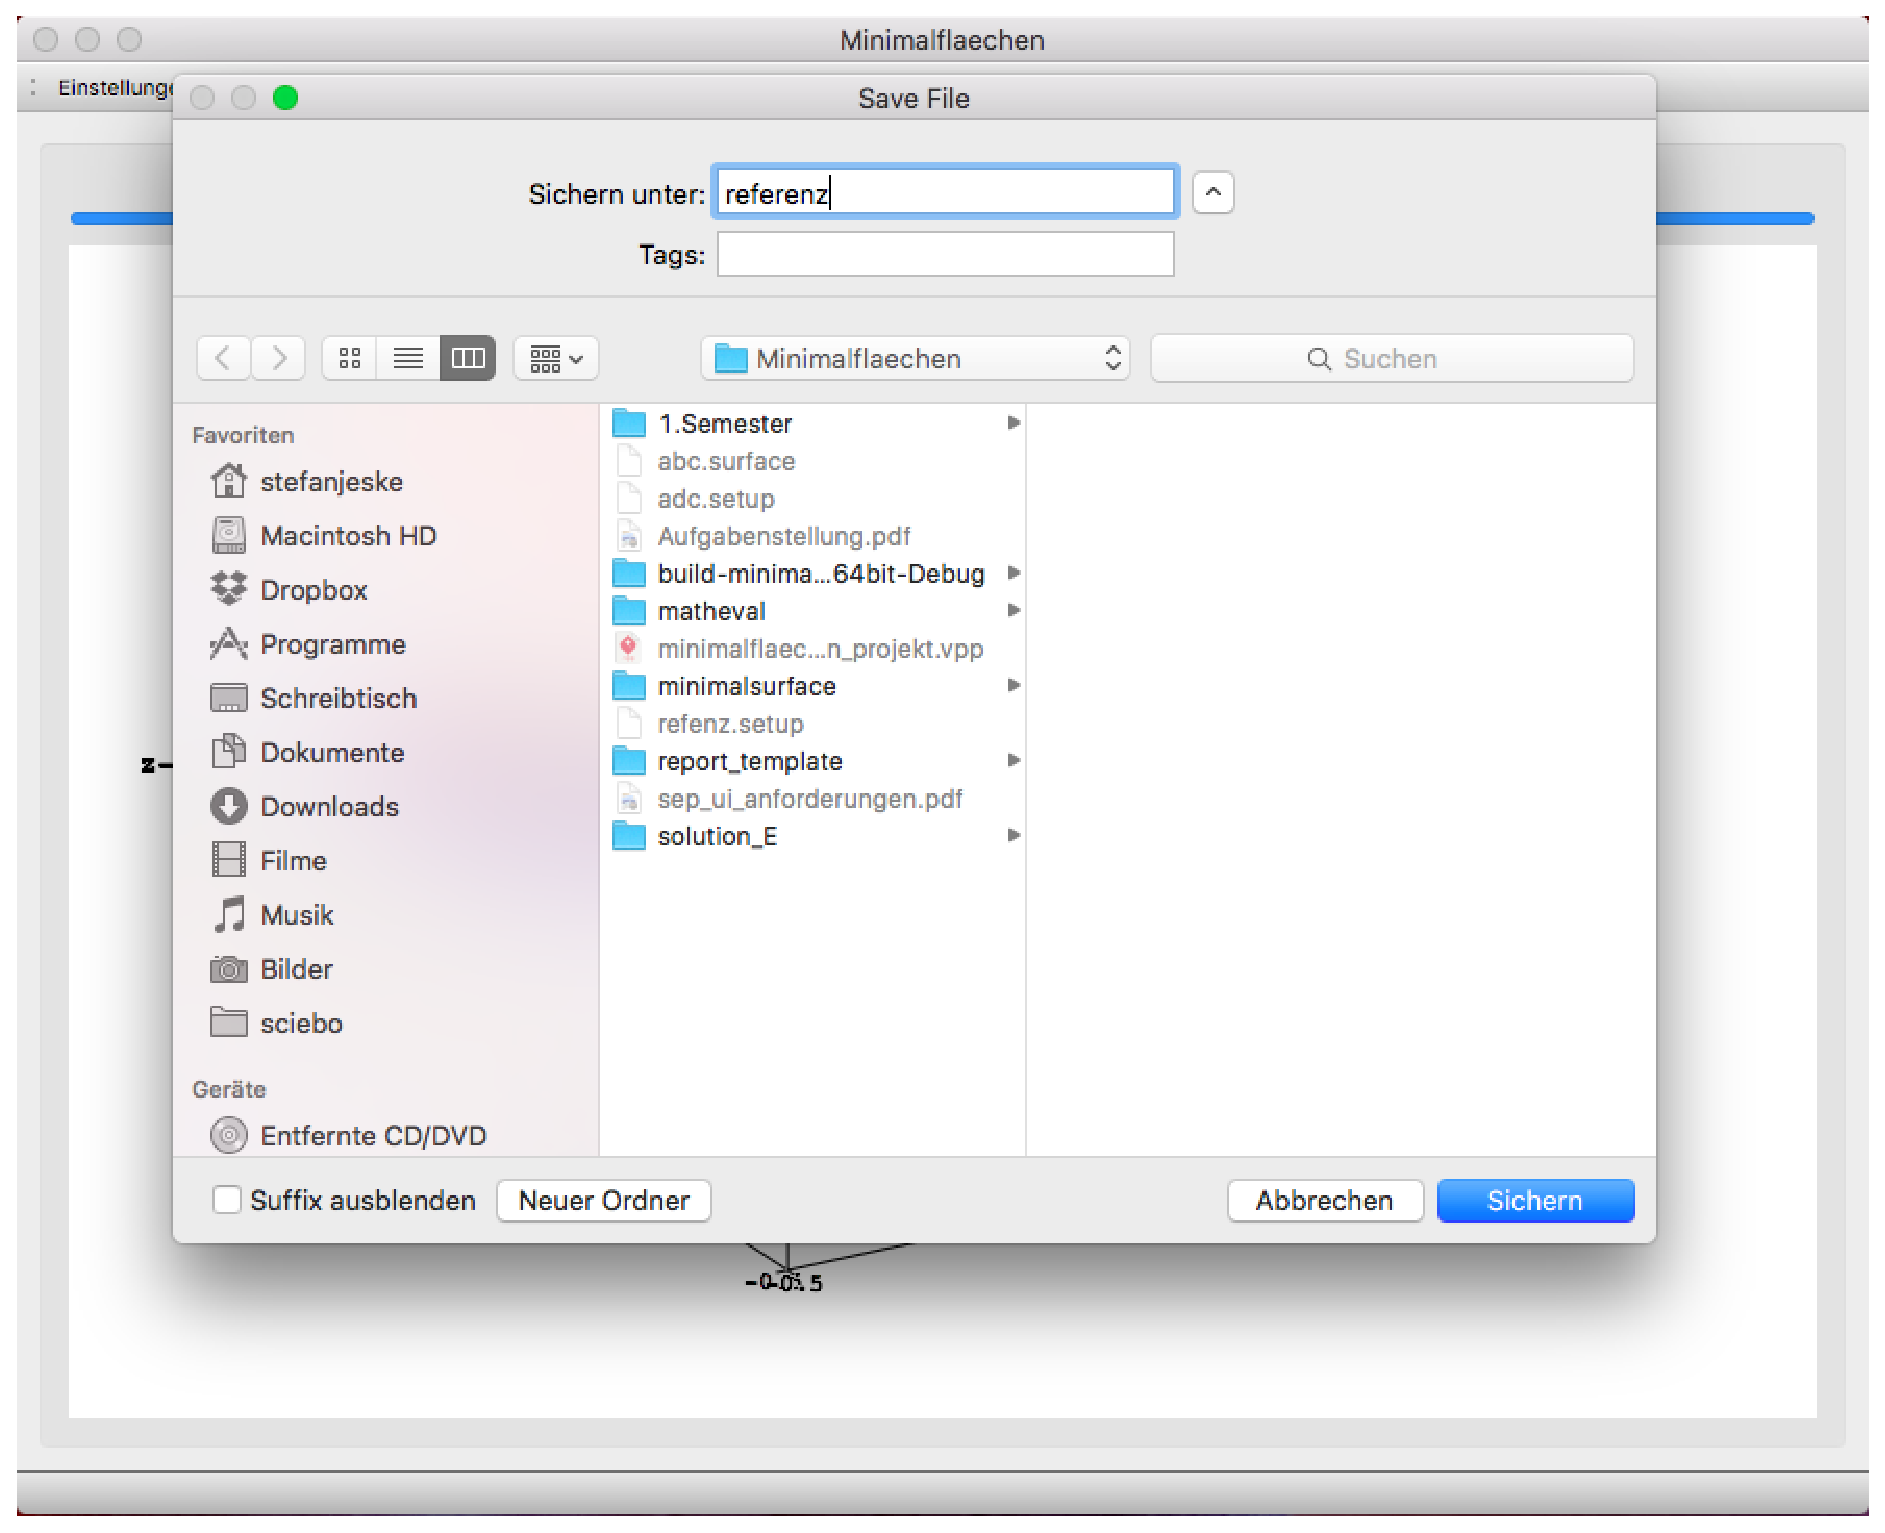
\includegraphics[width=\textwidth]{nutzerdoc/example_session/bsp_6}
\caption{Startbildschirm des Programms}
\end{figure}

Es wird der gew\"unschte Ordner zum Speichern ausgew\"ahlt und der Datei ein Name gegeben. Anschlie\ss end wird auf {\tt Sichern} geklickt, wodurch die berechneten Ergebnisse zur Weiterverwendung bereitstehen. \\
Abschlie\ss end wird das Programm durch Klicken auf den Button {\tt Quit} in dem {\tt Einstellungen} Tab beendet.

\section{Fehlersituationen}
Das Programm gibt Fehlermeldungen aus. Diese werden lediglich durch Fehler in den eingegebenen Funktionen, und durch ung�ltige Definitionsbereichsgrenzen hervorgerufen. \\
Funktionen erzeugen Fehler wenn sie nicht syntaktisch korrekt eingegeben werden, z.B. {\tt lug(x)} anstelle {\tt log(x)}.\\
F\"ur die Definitionsbereichsgrenzen muss lediglich gelten, dass die untere Grenze kleiner ist als die obere.\\
Sollten dennoch Fehler auftreten bitten wir diese an stefan.jeske@rwth-aachen.de zu melden. 
\chapter{Entwicklerdokumentation}
\label{ch:5}

\section{Codestruktur}
Der Code besteht aus mehreren Klassen. Die Quelldateien befinden sich gr\"o\ss tenteils im {\tt root} Verzeichnis. Die verwendeten Bibliotheken befinden sich in den Ordnern mit gleichem Namen. Siehe Kapitel 4 f\"ur Installation. Im Folgenden wird die Codestruktur im Groben beschrieben. F\"ur eine detaillierte Dokumentation siehe Abschnitt 2 in diesem Kapitel.

\subsection{Klasse MainWindow}
Die Klasse {\tt MainWindow} ist f\"ur die graphische Darstellung der Benutzeroberfl\"ache zust\"andig. Der Quellcode findet sich in \refsec{ssec:6.1.1} und in den Dateien {\tt mainwindow.h} und {\tt mainwindow.cpp}. Au\ss erdem wird in dieser Klasse das Laden und Speichern von Einstellung und Ergebnis definiert.

\subsection{Klasse Controller}
Die Klasse {\tt Controller} verwaltet die Berechnung des Ergebnisses. Sie steuert die Klasse {\tt Discretization}, welche auf einem anderen Thread rechnet, damit das Interface weiter verwendet werden kann.  Der Quellcode befindet sich in \refsec{6.1.2} und in den Dateien {\tt controller.h} und {\tt controller.cpp}.

\subsection{Klasse Paramter}
Die Klasse {\tt Parameter} ist komplett \"offentlich definiert. Es existiert zur Laufzeit immer maximal ein {\tt Parameter} Objekt welches per Referenz an alle Klassen vergeben, die dieses benötigen. Der Quellcode befindet sich in \refsec{6.1.3} und in den Dateien {\tt parameter.h} und {\tt parameter.cpp}.

\subsection{Klasse Discretization}
In der Klasse {\tt Discretization} ist die eigentliche Berechnung der Minimalfl\"ache unter Verwendung des Newton Verfahrens implementiert. Da {\tt Discretization} auf einem anderen Thread arbeitet als die anderen Klassen, existiert auch nur ein Objekt, welches erst nach der Beendung des Programms gel\"oscht wird. Der Quellcode befindet sich in \refsec{6.1.4} und in den Dateien {\tt discretization.h} und {\tt discretization.cpp}.

\subsection{Klasse Plot}
Die Klasse {\tt Plot} wird von der Klasse {\tt Qwt3D::SurfacePlot} abgeleitet, und stellt lediglich das Plot Widget zu Verf\"ugung. Der Quellcode befindet sich in \refsec{6.1.5} und in der Datei {\tt plot.h}.

\subsection{Hilfsfunktionen}
Die eigen definierten Hilfsfunktionen f\"ur den L\"oser befinden sich in \refsec{6.1.6} und in der Datei {\tt solverfunctions.h}

\section{Detaillierte Dokumentation des Codes}
In dem Unterverzeichnis {\tt ./minimalsurface/doc/} befindet sich die Konfigurationsdatei {\tt Doxyfile} f\"ur die Erstellung der doxygen Dokumentation in {\tt HTML} oder \LaTeX\ Format. Zum Erstellen der Dokumentation muss der Befehl {\tt doxygen Doxyfile} in dem Verzeichnis {\tt ./minimalsurface/doc/} aufgerufen werden. Es werden zwei neue Verzeichnisse {\tt ./minimalsurface/doc/html/} und {\tt ./minimalsurface/doc/latex/} erstellt. Um die {\tt HTML} Version anzuzeigen muss in den Ordner {\tt html} gewechselt werden und die Datei {\tt index.html} mit dem Standardbrowser ge\"offnet werden. Um die \LaTeX\ Dokumentation anzeigen zu lassen muss der Befehl {\tt make} in dem Ordner {\tt latex} ausgef\"uhrt werden. Anschlie\ss end kann die PDF Datei mit einem entsprechenden Programm gelesen werden.

\section{Software-Tests}
Alle Anwendungsf\"alle wurden manuell auf Funktionalit\"at getestet. Die folgenden Anwendungsf\"alle wurden erfolgreich ohne Fehlermeldungen getestet:
\begin{itemize}
	\item Beenden
	\item Tab wechseln
	\item Speichern
	\item Laden
	\item Einstellungen \"andern
\end{itemize}
Der Anwendungsfall Berechnung starten wurde erfolgreich mit allen Fehlersituationen getestet, die in der Benutzerdokumentation ausf\"uhrlicher beschrieben sind.

%\bibliographystyle{plain}
%\bibliography{analyse_entwurf}

\appendix

\chapter{Quellcode}
\label{ch:6}

{\em einfach referenzierbare Version des Quelltexts} 

\section{Paket 1}
\label{sec:6.1}

\subsection{Klasse 1.1}
\label{ssec:6.1.1}

\begin{lstlisting}[caption=Dokumentierter Quellcode in {\tt klasse1.1.hpp},label=klasse1.1.hpp]
class foo {
  public:
    int bar(const float& f); /*@\label{zn_bar}@*/
}
\end{lstlisting}

\subsection{Klasse 1.2}

\section{Paket 2}

\section{Paket 3}



\end{document}

